\documentclass[spanish,a4paper,12pt,oneside]{extreport}

\usepackage[dvips]{graphicx}
\usepackage[dvips]{epsfig}
\usepackage[utf8]{inputenc}
\usepackage[spanish]{babel}
\usepackage{alltt}
\usepackage[citestyle=apa,bibstyle=apa]{biblatex}

\usepackage[ruled,vlined,commentsnumbered,linesnumbered,inoutnumbered,titlenotnumbered,noend]{algorithm2e}
\SetKwRepeat{Do}{do}{while}

\usepackage{multirow}
\usepackage{array} 
\usepackage{amsfonts}
\usepackage{amsmath}
\usepackage{bigstrut}
\usepackage{booktabs}
\usepackage{caption}
\usepackage{chngpage}
\usepackage{float}
\usepackage{comment}
%\usepackage{enumitem,lipsum}
\usepackage{graphicx}
\usepackage{lscape}
\usepackage{microtype}
% \usepackage{natbib}
\usepackage{pdflscape}
\usepackage{rotating}
\usepackage{subcaption}
\usepackage{ctable}
\usepackage{hyperref}
\usepackage{enumerate}
\usepackage{gensymb}
\usepackage{eurosym}
\usepackage{xcolor}
\usepackage{tabu}
\usepackage[export]{adjustbox}[2011/08/13]
\usepackage{lineno}
\usepackage{epigraph}
%\usepackage[sanitize=none]{glossaries}
\usepackage{glossaries}

\usepackage{wrapfig}

%Define the listing package
\usepackage{listings} %code highlighter
\usepackage{color} %use color
\definecolor{mygreen}{rgb}{0,0.6,0}
\definecolor{mygray}{rgb}{0.5,0.5,0.5}
\definecolor{mymauve}{rgb}{0.58,0,0.82}
 
%Customize a bit the look
\lstset{ %
backgroundcolor=\color{white}, % choose the background color; you must add \usepackage{color} or \usepackage{xcolor}
basicstyle=\footnotesize, % the size of the fonts that are used for the code
breakatwhitespace=false, % sets if automatic breaks should only happen at whitespace
breaklines=true, % sets automatic line breaking
captionpos=b, % sets the caption-position to bottom
commentstyle=\color{mygreen}, % comment style
deletekeywords={...}, % if you want to delete keywords from the given language
escapeinside={\%*}{*)}, % if you want to add LaTeX within your code
extendedchars=true, % lets you use non-ASCII characters; for 8-bits encodings only, does not work with UTF-8
frame=single, % adds a frame around the code
keepspaces=true, % keeps spaces in text, useful for keeping indentation of code (possibly needs columns=flexible)
keywordstyle=\color{blue}, % keyword style
% language=Octave, % the language of the code
morekeywords={*,...}, % if you want to add more keywords to the set
numbers=left, % where to put the line-numbers; possible values are (none, left, right)
numbersep=5pt, % how far the line-numbers are from the code
numberstyle=\tiny\color{mygray}, % the style that is used for the line-numbers
rulecolor=\color{black}, % if not set, the frame-color may be changed on line-breaks within not-black text (e.g. comments (green here))
showspaces=false, % show spaces everywhere adding particular underscores; it overrides 'showstringspaces'
showstringspaces=false, % underline spaces within strings only
showtabs=false, % show tabs within strings adding particular underscores
stepnumber=1, % the step between two line-numbers. If it's 1, each line will be numbered
stringstyle=\color{mymauve}, % string literal style
tabsize=2, % sets default tabsize to 2 spaces
title=\lstname % show the filename of files included with \lstinputlisting; also try caption instead of title
}
%END of listing package%
 
\definecolor{darkgray}{rgb}{.4,.4,.4}
\definecolor{purple}{rgb}{0.65, 0.12, 0.82}
 
%define Javascript language
\lstdefinelanguage{JavaScript}{
keywords={typeof, new, true, false, catch, function, return, null, catch, switch, var, if, in, while, do, else, case, break},
keywordstyle=\color{blue}\bfseries,
ndkeywords={class, export, boolean, throw, implements, import, this},
ndkeywordstyle=\color{darkgray}\bfseries,
identifierstyle=\color{black},
sensitive=false,
comment=[l]{//},
morecomment=[s]{/*}{*/},
commentstyle=\color{purple}\ttfamily,
stringstyle=\color{red}\ttfamily,
morestring=[b]',
morestring=[b]"
}
 
\lstset{
language=JavaScript,
extendedchars=true,
basicstyle=\footnotesize\ttfamily,
showstringspaces=false,
showspaces=false,
numbers=left,
numberstyle=\footnotesize,
numbersep=9pt,
tabsize=2,
breaklines=true,
showtabs=false,
captionpos=b
}


%\\linenumbers
%\setlength\linenumbersep{5pt}
%\renewcommand\linenumberfont{\normalfont\tiny\sffamily\color{gray}}

%\makenoidxglossaries
\makeglossaries

\newglossaryentry{API}
{
    name=API,
    description={Una \textbf{interfaz de programación de aplicaciones} es una manera de que dos o más programas informáticos se comuniquen entre sí. Es un tipo de interfaz de software que ofrece un servicio a otras piezas de software}
}

\newglossaryentry{CLI}
{
    name=CLI,
    description={Es un tipo de interfaz de usuario de computadora que permite a los usuarios dar instrucciones a algún programa informático o al sistema operativo por medio de una línea de texto simple}
}

\newglossaryentry{CWD}
{
    name=CWD,
    description={CWD (Current Working Directory) se refiere al directorio actual en el que se está trabajando dentro de un sistema de archivos. Es la ubicación o carpeta en la que un programa o usuario se encuentra actualmente realizando operaciones o ejecutando comandos}
}

\newglossaryentry{JSX}
{
    name=JSX,
    description={Es una extensión de JavaScript que combina HTML y JavaScript para facilitar la creación de interfaces de usuario en aplicaciones web, especialmente en frameworks como React.}
}

\newglossaryentry{framework}
{
    name=framework,
    description={Un framework es una estructura de software que proporciona herramientas y bibliotecas para facilitar el desarrollo de aplicaciones. Actúa como una base sobre la cual se construyen aplicaciones, ahorrando tiempo al ofrecer soluciones predefinidas para tareas comunes. Los frameworks permiten a los desarrolladores enfocarse en la lógica de su aplicación en lugar de preocuparse por detalles de implementación, lo que agiliza el proceso de desarrollo y promueve la reutilización de código.}
}

\newglossaryentry{MPA}
{
    name=MPA,
    description={Multi-Page Application (MPA) se refiere a un tipo de aplicación web que consta de varias páginas individuales. Cada página representa una vista diferente de la aplicación y se carga por separado del servidor cuando el usuario navega entre ellas. A diferencia de las Single-Page Applications (SPA), que cargan una única página y actualizan su contenido de forma dinámica, las MPAs requieren una carga completa de cada página, lo que puede generar una experiencia más tradicional de navegación.}
}

\newglossaryentry{SSR}
{
    name=SSR,
    description={Server-Side Rendering (SSR) es un enfoque en el desarrollo web donde el servidor genera y envía la página completa al cliente como HTML listo para ser mostrado, ofreciendo una carga inicial más rápida.}
}

\newglossaryentry{SSG}
{
    name=SSG,
    description={SSG (Static Site Generation) es un enfoque de desarrollo web donde las páginas web se generan de antemano durante la compilación, lo que resulta en un rendimiento rápido y una menor carga en el servidor.}
}
\usepackage[top=2cm, bottom=2cm, left=2cm, right=2cm]{geometry}

\newenvironment{sourcecode}
{\begin{list}{}{\setlength{\leftmargin}{1em}}\item\scriptsize\bfseries}
{\end{list}}

\newenvironment{littlesourcecode}
{\begin{list}{}{\setlength{\leftmargin}{1em}}\item\tiny\bfseries}
{\end{list}}

\newenvironment{summary}
{\par\noindent\begin{center}\textbf{Abstract}\end{center}\begin{itshape}\par\noindent}
{\end{itshape}}

\newenvironment{keywords}
{\begin{list}{}{\setlength{\leftmargin}{1em}}\item[\hskip\labelsep \bfseries Keywords:]}
{\end{list}}

\newenvironment{palabrasClave}
{\begin{list}{}{\setlength{\leftmargin}{1em}}\item[\hskip\labelsep \bfseries Palabras clave:]}
{\end{list}}

\usepackage{bera}% optional: just to have a nice mono-spaced font
\usepackage{listings}
\usepackage{xcolor}

\colorlet{punct}{red!60!black}
\definecolor{background}{HTML}{EEEEEE}
\definecolor{delim}{RGB}{20,105,176}
\colorlet{numb}{magenta!60!black}

\lstdefinelanguage{json}{
    basicstyle=\normalfont\ttfamily,
    numbers=left,
    numberstyle=\scriptsize,
    stepnumber=1,
    numbersep=8pt,
    showstringspaces=false,
    breaklines=true,
    frame=lines,
    backgroundcolor=\color{background},
    literate=
     *{0}{{{\color{numb}0}}}{1}
      {1}{{{\color{numb}1}}}{1}
      {2}{{{\color{numb}2}}}{1}
      {3}{{{\color{numb}3}}}{1}
      {4}{{{\color{numb}4}}}{1}
      {5}{{{\color{numb}5}}}{1}
      {6}{{{\color{numb}6}}}{1}
      {7}{{{\color{numb}7}}}{1}
      {8}{{{\color{numb}8}}}{1}
      {9}{{{\color{numb}9}}}{1}
      {:}{{{\color{punct}{:}}}}{1}
      {,}{{{\color{punct}{,}}}}{1}
      {\{}{{{\color{delim}{\{}}}}{1}
      {\}}{{{\color{delim}{\}}}}}{1}
      {[}{{{\color{delim}{[}}}}{1}
      {]}{{{\color{delim}{]}}}}{1},
}

% Configuración de los colores de los enlaces
\hypersetup{
    colorlinks = true,
    linkcolor = blue,
    filecolor = magenta,      
    urlcolor = cyan,
}

\addbibresource{memtfg.bib}

\begin{document}

\renewcommand\listtablename{Índice de Tablas}    
\renewcommand\listfigurename{Índice de Figuras}    

%%%%%%%%%%%%%%%%%%%%%%%%%%%%%%%%%%%%%%%%%%%%%%%%%%%%%%%%%%%%%%%%%%%%%%%%%%%%%%%
% First Page
%%%%%%%%%%%%%%%%%%%%%%%%%%%%%%%%%%%%%%%%%%%%%%%%%%%%%%%%%%%%%%%%%%%%%%%%%%%%%%%
\pagestyle{empty}
\thispagestyle{empty}


\newcommand{\HRule}{\rule{\linewidth}{1mm}}
\setlength{\parindent}{0mm}
\setlength{\parskip}{0mm}

\vspace*{\stretch{0.5}}

\begin{center}

\includegraphics[scale=0.8]{images/escuela-ingenieria-tecnologia-original}\\[10mm]
{\Huge Trabajo de Fin de Grado}
\end{center}

\HRule
\begin{flushright}
        {\Huge AdAstra: Un Generador Estático de Sistemas de Gestión de Aprendizaje %(LMS)
        } \\[2.5mm]
        {\Large \textit{AdAstra: A Static Learning Management System Generator}} \\[5mm]
        {\Large Jaime Armas Rivero} \\[5mm]

\end{flushright}
\HRule
\vspace*{\stretch{2}}
\begin{center}
  \Large La Laguna, \today
\end{center}

\setlength{\parindent}{5mm}

%%%%%%%%%%%%%%%%%%%%%%%%%%%%%%%%%%%%%%%%%%%%%%%%%%%%%%%%%%
% Signature page (add the official stamp)
%%%%%%%%%%%%%%%%%%%%%%%%%%%%%%%%%%%%%%%%%%%%%%%%%%%%%%%%%%
\newpage
\thispagestyle{empty}

D. {\bf Casiano Rodríguez León}, con N.I.F. 42.020.072-S  profesor Catedrático de Universidad adscrito al Departamento de Ingeniería Informática y de Sistemas de la Universidad de La Laguna, como tutor


\bigskip
\bigskip
{\bf C E R T I F I C A}

\bigskip
\bigskip
Que la presente memoria titulada:

\bigskip
AdAstra: Un Generador Estático de Sistemas de Gestión de Aprendizaje
\bigskip
\bigskip
\bigskip

\noindent ha sido realizada bajo su dirección por D. {\bf Jaime Armas Rivero},
con N.I.F. 79084143T.

\bigskip
\bigskip

Y para que así conste, en cumplimiento de la legislación vigente y a los efectos
oportunos firman la presente en La Laguna a \today

%%%%%%%%%%%%%%%%%%%%%%%%%%%%%%%%%%%%%%%%%%%%%%%%%%%%%%%%%%
\newpage
\thispagestyle{empty}

%{ \flushright

\begin{LARGE}
Agradecimientos
\end{LARGE}

\hspace{3mm}

\begin{large}
A mi familia y amigos por aconsejarme, fortalecerme y confiar en mí.\\
\end{large}

%}
%%%%%%%%%%%%%%%%%%%%%%%%%%%%%%%%%%%%%%%%%%%%%%%%%%%%%%%%
\newpage
\thispagestyle{empty}

\bigskip
\begin{LARGE}
Licencia
\end{LARGE}

\begin{center}

\includegraphics[scale=1.8]{images/by_88x31}\\[5mm]
\end{center}

\begin{large}
© Esta obra está bajo una licencia de Creative Commons Reconocimiento 4.0 Internacional.
\end{large}

%%%%%%%%%%%%%%%%%%%%%%%%%%%%%%%%%%%%%%%%%%%%%%%%%%%%%%%%
\newpage 
\thispagestyle{empty}

\begin{abstract}
Es un hecho consolidado el uso de GitHub como plataforma para la enseñanza, especialmente en el ámbito de 
la Informática. 
La propia empresa  apoya estas iniciativas dentro de un grupo de acciones que se engloban 
bajo el término  GitHub Education y que incluye no solo descuentos, 
foros, congresos, becas, etc. sino también herramientas específicas para la educación como  GitHub Classroom, 
la cual da soporte al proceso de asignación de tareas.

Además, debido a la creciente popularización de las páginas web estáticas basadas en la metodología Jamstack
se está extendiendo cada vez más su uso y están saliendo nuevas tecnologías que se respalden en estas.

Este trabajo presenta una herramienta que permita generar LMS estáticos, facilitando el trabajo y configuración de los mismos.
Los LMS generados siguen metodologías y prácticas que son comunes en GitHub Education
y hacen uso de los servicios y herramientas que proporciona GitHub.
La cual se aprovechara de la API GraphQL de GitHub para conectarse con las tareas e información
dentro la organización creada por el profesor para impartir sus clases e incorporarlas dentro del LMS.

\begin{palabrasClave}
github-education, astro, github-classroom, graphql, git, javascript, typescript
\end{palabrasClave}

\end{abstract}
%%%%%%%%%%%%%%%%%%%%%%%%%%%%%%%%%%%%%%%%%%%%%%%%%%%%%%%%%
\newpage 
\vspace*{200px}
\thispagestyle{empty}

\begin{summary}
It is a consolidated fact the use of GitHub as a platform for teaching, especially in the field of Computer Science.
The company itself supports these initiatives within a group of actions that fall under the term GitHub Education,
which includes not only discounts, forums, conferences, scholarships, etc. but also specific tools for
education such as GitHub Classroom, which supports the task assignment process.

In addition, due to the growing popularity of static web pages based on the Jamstack methodology,
their use is increasingly widespread and new technologies that rely on them are emerging.

This work presents a tool that allows generating static LMS, facilitating their work and configuration.
The generated LMS follows methodologies and practices that are common in GitHub Education and
make use of the services and tools provided by GitHub. It will take advantage of the GitHub GraphQL API
to connect with the tasks and information within the organization created by the teacher to teach
their classes and incorporate them into the LMS.
\begin {keywords}
github-education, astro, github-classroom, graphql, git, javascript, typescript
\end {keywords}

\end{summary}
%%%%%%%%%%%%%%%%%%%%%%%%%%%%%%%%%%%%%%%%%%%%%%%%%%%%%%%%%
\newpage{\pagestyle{empty}}
\thispagestyle{empty}

%%%%%%%%%%%%%%%%%%%%%%%%%%%%%%%%%%%%%%%%%%%%%%%%%%%%%%%%%
\pagestyle{myheadings} %my head defined by markboth or markright
% No funciona bien \markboth sin "twoside" en \documentclass, pero al
% ponerlo se dan un montón de errores de underfull \vbox, con lo que no se
% ha puesto.


%%Aqui debería poner el nombre del proyecto pero, como es muy grande no cabe y se ve feo en el PDF
\markboth{xxxxx}{}

%%%%%%%%%%%%%%%%%%%%%%%%%%%%%%%%%%%%%%%%%%%%%%%%%%%%%%%%%
%Numeracion en romanos
\renewcommand{\thepage}{\roman{page}}
\setcounter{page}{1}
\pagestyle{plain} 

%%%%%%%%%%%%%%%%%%%%%%%%%%%%%%%%%%%%%%%%%%%%%%%%%%%%%%%%%

{\hypersetup{linkcolor=black}
\tableofcontents

%%%%%%%%%%%%%%%%%%%%%%%%%%%%%%%%%%%%%%%%%%%%%%%%%%%%%%%%%
\newpage{\pagestyle{empty}}

\listoffigures

%%%%%%%%%%%%%%%%%%%%%%%%%%%%%%%%%%%%%%%%%%%%%%%%%%%%%%%%%
\newpage{\pagestyle{empty}}

\listoftables
}

%%%%%%%%%%%%%%%%%%%%%%%%%%%%%%%%%%%%%%%%%%%%%%%%%%%%%%%%%%%%%%%%%%%%%%%%%%%%%%%
\newpage{\pagestyle{empty}}

%%%%%%%%%%%%%%%%%%%%%%%%%%%%%%%%%%%%%%%%%%%%%%%%%%%%%%%%%%%%%%%%%%%%%%%%%%%%%%%
\newpage
\thispagestyle{empty}

%Numeracion a partir del capitulo I
\renewcommand{\thepage}{\arabic{page}}
\setcounter{page}{1}
\pagestyle{plain}

\chapter{\LARGE Introducción, Antecedentes y Estado del Arte}
\label{chapter:intro}

%\section{Motivación}
\section{Introducción}
%Repetir aquí el proyecto de TFG
Durante muchos años, profesores de programación de todo el mundo han utilizado y siguen utilizando GitHub como plataforma para la enseñanza de asignaturas relacionadas con la programación, el trabajo en equipo y el desarrollo de proyectos. La propia empresa GitHub ha apoyado estas iniciativas dentro de un grupo de acciones que se inscriben bajo el término  GitHub Education. Ello incluye descuentos en plataformas y herramientas para profesores y alumnos, foros específicos de discusión, congresos, becas, y herramientas específicas. Entre estas últimas cabe señalar  GitHub Classroom, la cual da soporte al proceso de asignación de tareas.

Hace solo dos años GitHub introdujo una herramienta denominada GitHub CLI (a veces referenciada como gh-cli o gh). Es una herramienta de código abierto para utilizar los servicios que provee GitHub, pero desde la línea de comandos.  Es posible ver, crear, clonar, y bifurcar repositorios; crear, cerrar, editar y ver incidencias, etc. Sin embargo el conjunto de funcionalidades  ofrecido es aún bastante menor que el disponible en la interfaz web.

En agosto del año 2021 los desarrolladores de GitHub Cli añadieron un mecanismo denominado gh-cli extensions (denominado gh-extensions) que facilita que terceros puedan añadir nuevas funcionalidades a gh-cli mediante un repositorio GitHub.
En el contexto específico de GitHub Education, las gh-extensions abren nuevas posibilidades para  proveer comandos que facilitan el flujo de trabajo diario de los profesores y alumnos y que pueden ser de uno de estos tipos:
\begin{itemize}
  \item Creación y manejo de las organizaciones GitHub asociadas a las asignaturas
  \item Creación y manejo de asignaciones de tareas dentro de una asignatura
  \item Obtención de información sobre las actividades de los alumnos
  \item Facilitar la respuesta pronta a las dudas 
  \item Facilitar la elaboración de propuestas de mejora a los trabajos realizados por los alumnos
  \item Mejorar la eficiencia en los procesos de evaluación 
\end{itemize}

\section{Antecedentes y estado actual del tema}
Uno de los primeros intentos en integrar GitHub al mundo educativo fue \href{https://github.com/education/teachers_pet}{“teachers\_pet”}, una herramienta de la línea de comandos que ayudaba al profesorado a impartir sus clases intentando emular una plataforma de aprendizaje. Cada clase era una organización de GitHub y los alumnos estaban repartidos en equipos en los que estaban solo ellos mismos, de esta manera los profesores podían gestionar todos los repositorios de la organización, dar plantillas con las que los alumnos podían empezar a trabajar, comprobar el progreso, etc.
 Más tarde, GitHub respondería a la demanda con Github Classroom  un servicio web de uso más intuitivo que dejaría obsoleto a \verb|teacher's pet|, y que a día de hoy es la más utilizada.

En lo referente al GitHub CLI ya existía con anterioridad, una herramienta antecesora similar que proveía funcionalidades similares, fue  llamada \verb|hub|, actualmente mantenida por Mislav Marohnić (empleado de GitHub, Inc.). Hub fue creado originalmente por Chris Wanstrath, que junto con Tom Preston, Scott Chacon y P.J. Hyett fundaron GitHub en 2008. al igual que GitHub CLI esta herramienta nos permite interactuar con Github desde la terminal, pero esta se podría considerar un producto personal y más centrado en los denominados \gls{power users}. El 20 de febrero de 2020 Github anuncia Github CLI, el sucesor de hub mantenido y en desarrollo por un equipo oficial de la compañía y más amigable de usar. El 20 de agosto de 2021 sale la versión 2.0 con el comando \verb|extension|\cite{gh-extension}, con la cual los usuarios podrán crear sus propias extensiones que nos permiten generar por nosotros mismos y con relativa facilidad servicios y herramientas que se integren bien con las implementaciones actuales usando  las \gls{API}s de GitHub \verb|REST API|\cite{github-rest-api} y GitHub GraphQL\cite{github-graphql}.

Actualmente, existen cientos de extensiones dirigidas al desarrollador, pero son pocas las que están dedicadas a facilitar la gestión de las organizaciones, en especial aquellas dedicadas a la enseñanza. Este proyecto tiene como objetivo crear una extensión modular de GitHub CLI que complementa a GitHub classroom y que provee funcionalidades como:

\begin{itemize}
    \item Creación y asignación de tareas
    \item Seguimiento del progreso de los miembros de la organización
    \item Soporte a la gestión de incidencias
    \item Facilitar la retroalimentación a los trabajos realizados por los alumnos
    \item Interoperabilidad entre subcomandos para permitir comportamientos más complejos
    \item Interfaz rápida y amigable
\end{itemize}

%%%%%%%%%%%%%%%%%%%%%%%%%%%%%%%%%%%%%%%%%%%%%%%%%%%%%%%%%%%%%%%%%%%%%%%%%%%%%%%
\newpage{\pagestyle{empty}}
\thispagestyle{empty}

\chapter{\LARGE Tecnologías}
\label{chapter:dos}

La oferta de tecnologías a la hora de realizar un proyecto software es realmente extensa. A menudo la elección de estas tecnologías para formar la pila de desarrollo está vagamente justificada y el mayor argumento suele ser la familiaridad de los desarrolladores con las herramientas escogidas. Esto, de hecho, no es un argumento menor, ya que en un entorno real, adquirir los conocimientos suficientes sobre una serie de tecnologías como para crear un producto listo para la explotación necesita una gran cantidad de tiempo por parte del equipo de desarrollo y por ende también supone un importante costo económico. Sin embargo, sí que deberían conocerse los puntos débiles y fuertes de las principales opciones y debería realizarse un análisis para evitar problemas graves en el futuro. En este capítulo se describen las tecnologías empleadas para la realización de este proyecto y la justificación de la elección realizada. No se listan dependencias triviales, y que tengan un propósito inmediato (leer ficheros, crear archivos temporales, etcétera).


\section{GitHub}
GitHub es uno de los ejes centrales de todo este trabajo. A pesar de que no sea una plataforma enfocada en la enseñanza, es innegable el valor y productividad que proporcionada a virtualmente todos los desarrolladores de software del mundo. Los profesores pueden gestionar las clases en el mismo ámbito en el que se desarrollan las prácticas o tareas, y con la herramienta desarrollada mejorar la interacción tanto de profesores como de alumnos de los datos guardados en los repositorios de GitHub Classroom.

\subsection{Las APIs de GitHub: REST y  GraphQL}
Las \verb|API|s que nos proporciona GitHub son completamente necesarias. Sin ellas no podríamos tener ningún tipo de comunicación con los servicios de GitHub.

Se proveen dos APIs: \verb|API REST|\cite{github-rest-api} y GraphQL\cite{github-graphql}. En este trabajo se hace mayormente uso de la \verb|API GraphQL|. Se ha decidido de esta forma, pues con \verb|GraphQL| podemos obtener solo los datos que queremos, y podemos recibir en una única llamada información que de otra forma requeriría varías llamadas a diferentes \emph{endpoints}.

\section{Los Lenguajes JavaScript y TypeScript}
El lenguaje de programación escogido es \verb|JavaScript|\cite{js} (a partir de ahora \verb|JS|), más concretamente su extensión \verb|Typescript|\cite{ts} (a partir de ahora \verb|TS|). Los motivos son variados. Por un lado, es uno de los lenguajes con el que tengo más experiencia y destreza programando. A su vez, si tenemos en cuenta que en el lado de desarrollo web tanto \verb|TS|\cite{ts} como \verb|JS|\cite{js} es uno de sus mayores pilares es normal entender su uso.

Dejando de lado su popularidad y centrándonos en propiedades más intrínsecas del lenguaje, podemos ver que no hay mejor lenguaje para el manejo de ficheros JSON (usado por las API de GitHub), también al ser un lenguaje interpretado y flexible me ha permitido ser muy productivo en la fase de diseño y prototipado.

Se ha decidido usar \verb|TS| \cite{ts} antes que \verb|JS|\cite{js}, con el objetivo de minimizar bugs y aprovechar una mejor integración con editores de texto compatibles con: autocompletado inteligente, saltos a referencias, refactorización, etc.

No obstante, TypeScript es un lenguaje compilado y como tal requiere de su propio compilador. 
Esto añadiría otra dependencia al sistema aparte, aunque a día de hoy muchos frameworks y herramientas proveén de soporte directo de este facilitando el uso a los propios usuarios. 

En cuanto a dependencia de desarrollo, se ha usado como gestor de paquetes \verb|pnpm|\cite{pnpm} ya que se ha planteado usar un monorepo para almacenar todo los paquetes e aplicaciones de la herramienta y a día de hoy  \verb|pnpm|\cite{pnpm} es uno de los mejores gestores de paquetes que se integren con estos.

\section{El Lenguaje \LaTeX{} y Overleaf}
Para la elaboración de este documento se ha usado \LaTeX{}, 
en específico la implementación de \href{https://www.overleaf.com/}{overleaf}\cite{overlife}.
Gracias a esto hemos podido sincronizar con GitHub,
mantener un historial del documento, 
se ha simplificado la instalación de paquetes  y 
tenemos una copia accesible en línea que se sincroniza automáticamente.

\section{El sistema de compilación Turborepo}
El manejo de un monorepo para almacenar todas las aplicaciones y paquetes relacionados con la herramienta que se está desarrollando puede ser un desafío en términos de gestión de dependencias y versiones. Para abordar este problema, se ha utilizado \verb|TurboRepo|\cite{turborepo}, una tecnología que facilita el manejo de monorepos a gran escala.

TurboRepo es una herramienta de gestión de monorepos que se integra con el sistema de control de versiones Git. Proporciona una solución eficiente y escalable para el manejo de dependencias y versiones de múltiples aplicaciones y paquetes que se encuentran en el mismo repositorio. Al usar TurboRepo, se pueden configurar y administrar fácilmente las dependencias entre diferentes aplicaciones y paquetes, y también se puede realizar una gestión más efectiva de las versiones de cada uno de ellos.

Además, TurboRepo proporciona otras funcionalidades, como la capacidad de crear y publicar paquetes, y de gestionar la compilación y el despliegue de las aplicaciones. Todo esto se puede hacer de forma automatizada y con una gran flexibilidad.

En resumen, TurboRepo ha sido una elección clave para el manejo del monorepo que contiene todas las aplicaciones y paquetes relacionados con la herramienta que se está desarrollando. Su capacidad de gestionar dependencias y versiones a gran escala ha sido fundamental para mantener un proceso de desarrollo eficiente y escalable.

\section{El framework Astro}
Astro es una tecnología de construcción de aplicaciones web que se ha utilizado en este proyecto. Esta herramienta ofrece una solución moderna y rápida para el desarrollo de aplicaciones web basada en la idea de aplicaciones \verb|Multipaginas|\cite{multipage} y cero \verb|JS|\cite{js} dee forma predeterminada, permitiendo una integración fácil y eficiente con otras tecnologías y frameworks.

Una de las principales ventajas de Astro es su capacidad para generar sitios web altamente optimizados y rápidos, esto es gracias a que principalmente es un framework de modelo \verb|SSG|\cite{ssg} cuya principal idea es enviar cero \verb|JS|\cite{js} al cliente a menos que se requiera de dar interactividad, aunque esto no quita que este permita realizar \verb|SSR|\cite{ssr}. Además, Astro cuenta con una sintaxis intuitiva y fácil de usar, lo que la hace accesible para los desarrolladores con diferentes niveles de experiencia.

\subsection{Aplicación de múltiples páginas}
Astro usa un arquitectura de \verb|Aplicación de múltiples páginas|\cite{multipage} en el que un sitio web que consta de varias páginas HTML, en su mayoría renderizadas en el servidor. Cuando navegas a una nueva página, tu navegador solicita una nueva página de HTML al servidor.

\subsection{Soporte de multiples frameworks}
Una de las cosas por la que más destaca Astro, es que es una herramienta que esta diseñada para ser completamente personalizable y agnóstica a cualquier framework. Esto permite el uso de componentes de otros frameworks para diseñar la aplicaciones web. Además permite seleccionar si eso componentes se quieren usar solo para añadir diseño a las páginas o para añadir interactividad a través de su arquitectura de \verb|islas de componentes|\cite{islas}.

\subsection{Arquitectura de islas}
Como se menciono anteriormente Astro presenta un modelo de arquitectura de \verb|islas de componentes|\cite{islas} (el cual vamos a llamar \verb|Astro Islands|). Un \verb|Astro Island| se refiere a un componente de UI interactivo en una página HTML predominantemente estática. Pueden existir varias islas en una página, y una isla siempre se renderiza en forma aislada. Piensa en ellos como islas en un mar de HTML estático y no interactivo.

En Astro puedes utilizar cualquier framework de componentes de UI (React, Svelte, Vue, etc.). La técnica en la que se basa este patrón de arquitectura se conoce como hidratación parcial o selectiva a través de directivas que se añaden a los componentes de UI para señalar como quieren ser renderizados. Astro aprovecha esta técnica para hidratar las islas automáticamente.

\subsection{Rutas de API}
% Hablar de JAMstack pero se expande en diseño
En este framework el mayor modelo de uso es de \verb|SSG|\cite{ssg}, aunque también permite realizar \verb|SSR|\cite{ssr}. Este segundo de normal haría que la aplicación empezara a renderizar cada ruta directamente desde el servidor por petición de esta, lo cual no concuerda con lo planteado anteriormente que se dijo que se usaría renderizado estático para generar la aplicación. Aqui es donde entra una de las nuevas características añadidas por Astro recientemente que es el \verb|renderizado hibrido|\cite{hibrid}, la cual permite definir si una ruta se debe prerenderizar de manera estática aunque se este utilizando el \verb|SSR|\cite{ssr}.

\subsection{La sintexis MDX}
De base Astro incluye soporte para archivos \verb|Markdown|\cite{md}, los cuales se usan comúnmente para crear contenido con mucho texto, como artículos de blog y documentación. Aunque estos presentán un problema de base y es que si se quiere dejar que el usuario escriba su contenido facilmente y facilitarle le reutilización de material o usar más funcionalidades de las que ya ofrece \verb|Markdown|\cite{md}. Es por esto que se ha obtado por usar unos de los plugins disponibles en \verb|Astro|\cite{astro}, \verb|MDX|\cite{mdx}, el cual combina lo ya existente de \verb|Markdown|\cite{md} con nuevas funcionalidades como usar sintaxis como \verb|JSX|\cite{jsx} o expresiones \verb|JS|\cite{js}.

\subsection{La librería de autenticación astro-auth}
Viendo si la librería esta deprecada.

\section{El framework SolidJS}

\section{La librería Tailwindcss}


%%%%%%%%%%%%%%%%%%%%%%%%%%%%%%%%%%%%%%%%%%%%%%%%%%%%%%%%%%%%%%%%%%%%%%%%%%%%%%%
\newpage{\pagestyle{empty}}
\thispagestyle{empty}

\chapter{\LARGE Modo de uso}
\label{chapter:modo-de-uso}

En este capítulo se explicara una guía detallada paso a paso de como crear y desplegar un LMS con esta aplicación. En los capítulos siguientes se entrará en más detalle con respecto a la toma de decisiones en el diseño y como se ha logrado implementar todo la aplicación.

\section{Instalar node y un instalador de paquetes de JS}

Lo primero será descargar lo necesario para crear una aplicación que use javascript, en este caso, se deberá instalar node, con el siguiente link \url{https://nodejs.org/en/download} para Windows y Mac y en caso de usar una distribución de Linux el siguiente \url{https://nodejs.org/en/download/package-manager}. Esta instalación de normal ya trae incluido el instalor de paquetes \textbf{npm}, el cual se usará para los posteriores ejemplos. Si se desea instalar otro como pnmn\cite{pnpm} o yarn\cite{yarn}, habría que seguir la propia instalación de cada uno.

\section{Crear un Classroom de GitHub}

Esta aplicación esta centrada en la filosofía de enseñanza de GitHub, es por esto que lo primero que se deberá hacer es crear un GitHub Classroom, una herramienta para la enseñanza de GitHub. Para empezar se debera crear una cuenta de GitHub como se especifica aquí \url{https://docs.github.com/es/get-started/signing-up-for-github/signing-up-for-a-new-github-account}. Tras haber creado una cuenta de GitHub se podrá proceder a crear el Classroom, siguiendo la siguiente guía 

\url{https://docs.github.com/es/education/manage-coursework-with-github-classroom/teach-with-github-classroom/manage-classrooms}.

\section{Empezar una LMS con {\tt AdAstra}: create-adastra-lms}

Para empezar a usar el generador de LMS se deberá usar el comando \verb|npm create|\ref{npmCreate}, este comando esta presente en todo los instaladores de paquetes de JS y permite iniciar un proyecto, opcionalmente pasándole el paquete que se quiere usar para la creación. En este caso, se ha creado un paquete para que el usuario pueda iniciar un proyecto con AdAstra con nombre \textbf{create-adastra-lms}. Hay que destacar que en Windows debido a que la plantilla del proyecto usa links simbólicos, se deberá usar un terminal con permisos de administrador para ejecutar el comando. Para poder usar este paquete como inicializador se deberá usar el siguiente comando:
\begin{verbatim}
    npm create adastra-lms@latest
\end{verbatim}

Tras llamar a este comando se iniciará una aplicación de \verb|CLI|\cite{cli}, que preguntará sobre las opciones a querer usar. En este caso, lo que habrá que rellenar será lo siguiente:

\begin{enumerate}
    \item Directorio de la aplicación.
    \item Plantilla a usar. En este caso, solo esta la básica por lo que se deberá usar esa.
    \item Si se quiere instalar las dependencias.
    \item Si se quiere crear un repositorio de \verb|git|\ref{git}.
\end{enumerate}

En la figura \ref{fig:create-adastra} se  muestra un ejemplo de este proceso.

\begin{figure}
    \centering
    \makebox[\textwidth][c]{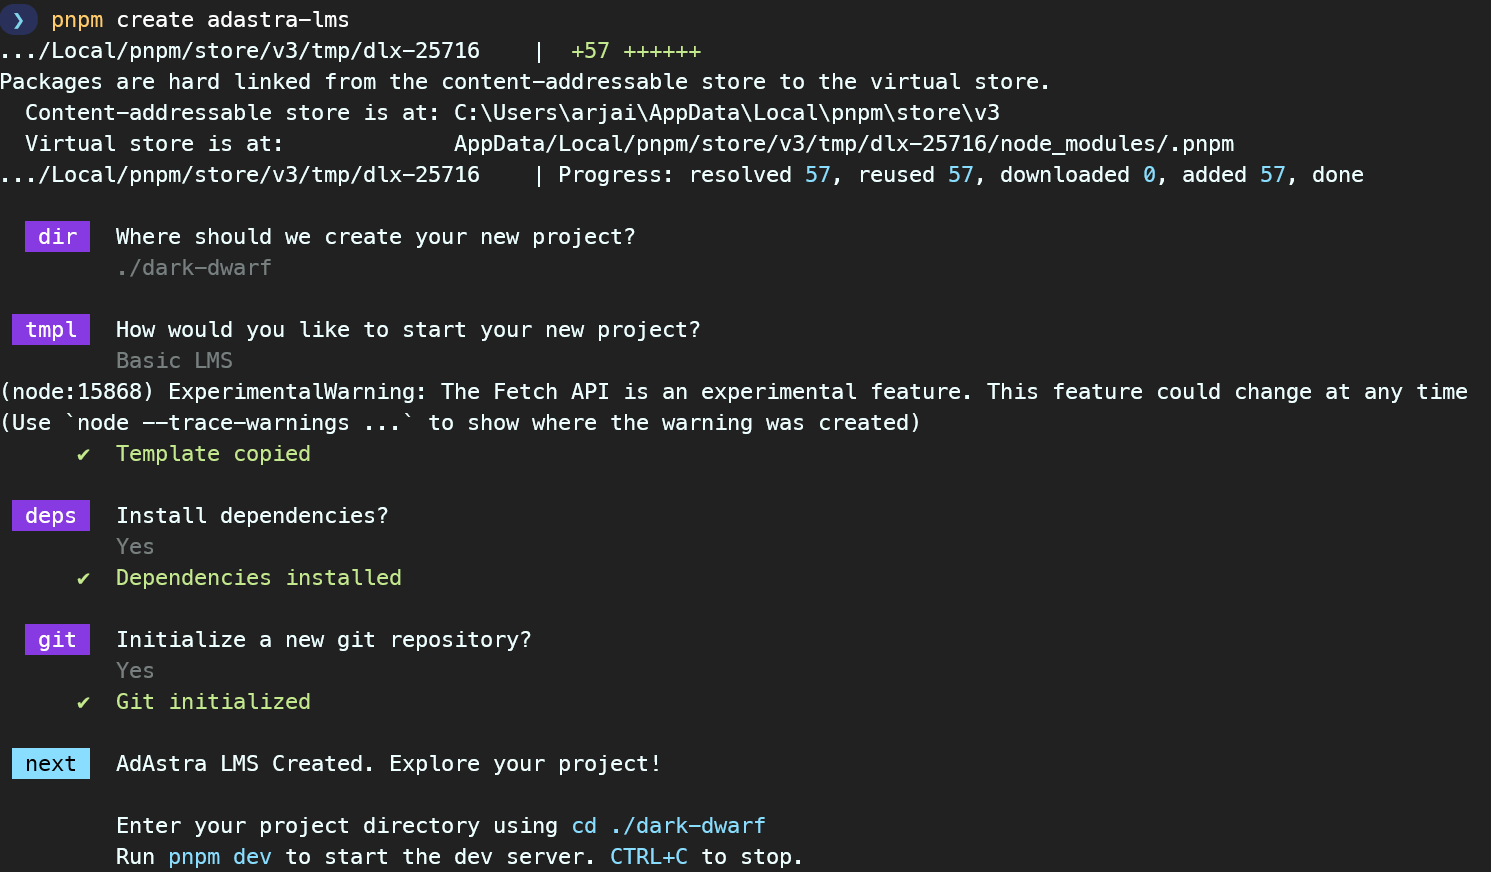
\includegraphics[width=\textwidth]{images/create-adastra-end.png}}
    \caption{Pasos de la ejecución del paquete create-adastra-lms}
    \label{fig:create-adastra}
\end{figure}

Tras usar este comando se creará un proyecto con la estructura mostrada en la figura \ref{fig:adastra-structure}.

\begin{figure}[H]
    \centering
    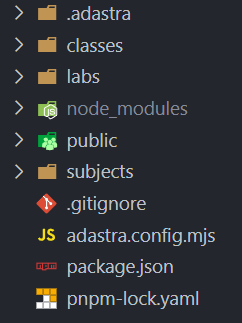
\includegraphics{images/projectStructure.png}
    \caption{Estructura de un proyecto creado con create-adastra-lms}
    \label{fig:adastra-structure}
\end{figure}

\section{Configuración del LMS}
El primer paso a seguir tras crear el proyecto será configurarlo. Hay dos pasos a seguir, 
primero actualizar el archivo de configuración de adastra (\verb|adastra.config.mjs|) y segundo
añadir las variables de entorno necesarias para el proyecto. Un ejemplo del archivo \verb|adastra.config.mjs| sería el que muestra en la figura \ref{fig:adastraConfig}

\subsection{Archivo de configuración: {\tt adastra.config.mjs}}

 Para esto habrá que modificar el archivo \textbf{adastra.config.js} que se ha creado automáticamente. Dentro de este se podrán encontrar dos objetos, el primero llamado \textbf{tailwindConfig} que se puede ver en la figura \ref{fig:adastraConfig} en la linea 1, el cual permitirá cambiar configuraciones relacionadas con el tema de la página que se creará como los colores primarios y secundarios, teniendo cada uno su opción para el estilo oscuro de la página, o incluso el tamaño que asignar al espaciado mínimo o la altura del navbar, etc. Esto funciona con la configuración de tailwindcss como base, en la documentación de tailwindcss (\url{https://tailwindcss.com/docs/theme}) se puede encontrar más información sobre esto. Y un segundo, llamado \textbf{organizationInfo} que se puede ver en la figura \ref{fig:adastraConfig} en la linea 24, dentro de este habrá que aportar información relacionada con la organización. Entre ellos los datos más importantes a introducir serían los siguientes:

 \begin{itemize}
    \item \textbf{pageTitle:} Titulo que aparecerá en la aplicación
    \item \textbf{github:} Objeto de configuración sobre GitHub
        \begin{itemize}
            \item \textbf{organizationName(obligatorio):} El nombre de la organización en GitHub.
            \item \textbf{classroomUrl:} Url del Classroom creado anteriormente.
        \end{itemize}
    \item \textbf{virtualCampus:} Objeto de configuración sobre el campus virtual
        \begin{itemize}
            \item \textbf{teachingGuideUrl:} Url a la guia docente de la asignatura
            \item \textbf{campusUrl:} Url al campus virtual de la asignatura
            \item \textbf{labsUrl:} Url a las tareas de la asignatura
        \end{itemize}
\end{itemize}

\begin{figure}
  \begin{lstlisting}[language=Javascript]
        export const tailwindConfig = {
          theme: {
            extend: {
              colors: {
                primary: "rgb(51 153 255 / <alpha-value>)",
                "dark-primary": "rgb(51 153 255 / <alpha-value>)",
                secondary: "rgb(135 45 230 / <alpha-value>)",
                "dark-secondary": "rgb(135 45 230 / <alpha-value>)",
                ...
              },
              spacing: {
                "navbar-height": "6rem",
                "sidebar-width": "18rem",
                ...
              },
              fontSize: {
                code: "1rem",
                ...
              },
            },
          },
        };
        
        export const organizationInfo = {
          pageTitle: "Test Asignatura",
          github: {
            organizationName: "ULL-ESIT-PL-2122",
            classroomUrl: "",
          },
          virtualCampus: {
            teachingGuideUrl: "",
            campusUrl: "",
            labsUrl: "",
          },
        };
    \end{lstlisting}
    \caption{Ejemplo del archivo de configuración de AdAstra: adastra.config.mjs}
    \label{fig:adastraConfig}
\end{figure}

\subsection{Configurar las variables de entornos}

Además para que la aplicación pueda obtener datos de la organización desde la API GraphQL de GitHub se tendrá que añadir a las variables de entorno del programa un token de acceso personal de GitHub \url{https://github.com/settings/tokens}, llamándolo \textbf{GITHUB\_SECRET}, en la figura\ref{fig:scopes} se muestra los \verb|scopes| que necesitará el token. La manera normal de añadir este secreto es a través de un \verb|.env| en el desarrollo y a la hora de hacer el despliegue de la aplicación habría que añadirlo a las variables de entorno del servicio. Por ejemplo, si se usa \verb|Vercel|\cite{vercel} como plataforma para el despliegue de la aplicación en la sección de \textit{Settings} hay un apartado llamado 
\textit{Environment Variables} en el que se pueden añadir variables de entornos a la aplicación. En la figura \ref{fig:vercelEnv} se puede ver de forma más detallada este menú.

\begin{figure}[H]
    \centering
    \makebox[\textwidth][c]{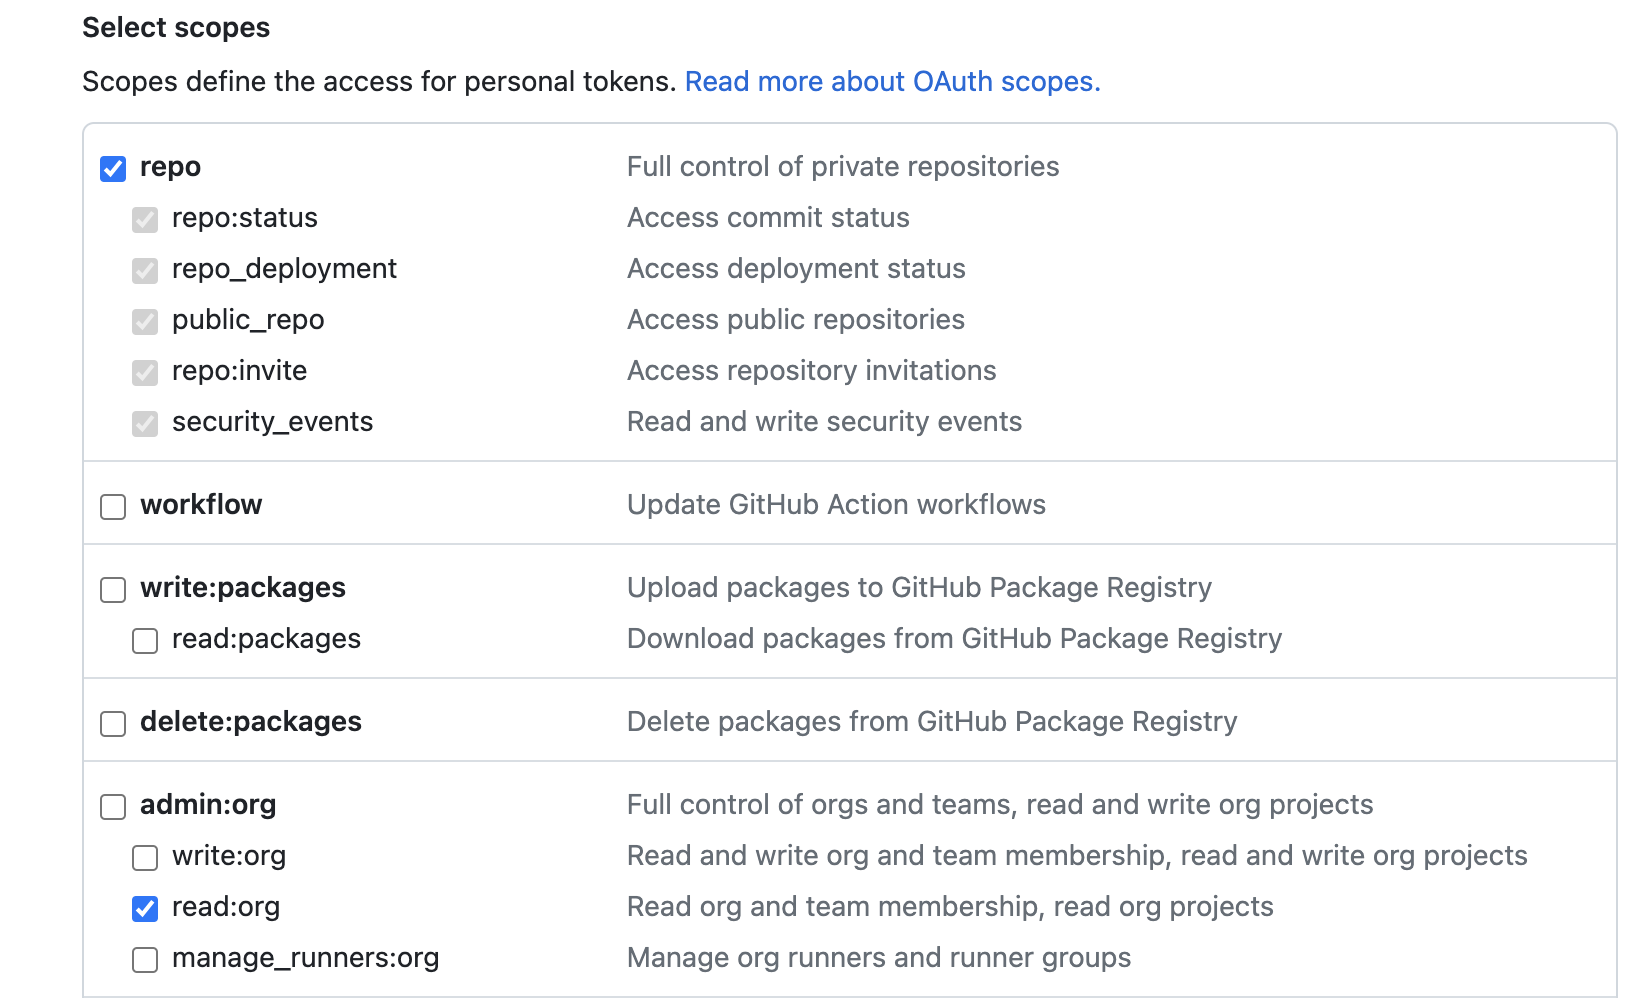
\includegraphics[width=\textwidth]{images/scopes.png}}
    \caption{Scopes para el token GITHUB\_SECRET}
    \label{fig:scopes}
\end{figure}

Ahora que ya está configurado podremos iniciar el proyecto localmente con el comando:
\begin{verbatim}
    npm run dev
\end{verbatim}

\begin{figure}[H]
    \centering
    \makebox[\textwidth][c]{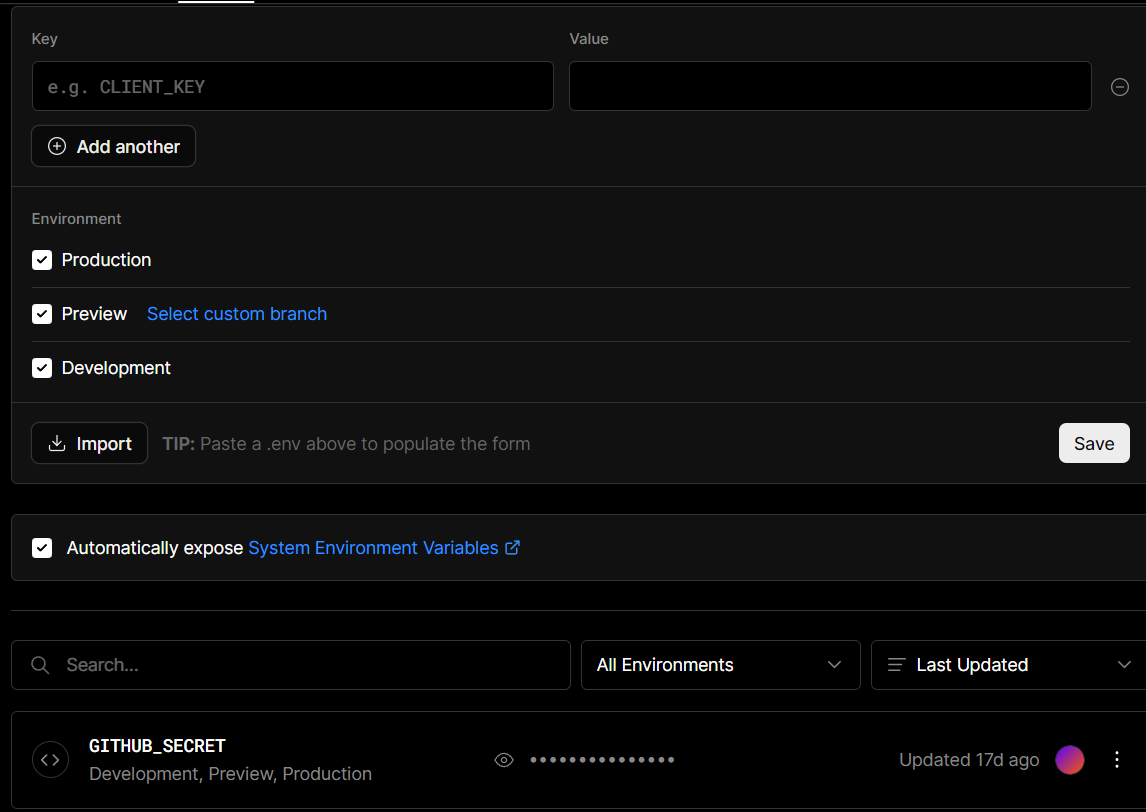
\includegraphics[width=\textwidth]{images/vercelEnv.png}}
    \caption{Menú para las variables de entorno en Vercel}
    \label{fig:vercelEnv}
\end{figure}

\section{Añadir contenido al LMS}

En cuanto al contenido habrá que diferenciar en cuatro tipos, elementos generales que se comparten entre todos los contenidos como imagenes, videos, archivos, etc; prácticas(labs), temarios(subjects) y clases(classes).

\subsection{Contenido general: {\tt public}}

El primer tipo de contenido, como se dijo anteriormente están relacionados con elementos que se quiera acceder en el resto de manera general, un ejemplo una imagen, y de base no modifican la pagina web que se crea, sino que sirven para expandir el tipo de información a poder usar en los contenidos posteriores. Por esto se proporciona una carpeta llamada \textbf{public}. Para poder acceder a estos elementos a posterior, se deberán usar accesos absolutos respecto a la carpeta public. Unos ejemplos serían estos:

\begin{verbatim}
    public/test.png -> /test.png
    public/images/test.png -> /images/test.png
\end{verbatim}

\subsection{Añadir un temario}

El primer contenido que deberá ser escrito por el usuario directamente y que realizará un cambio explicito en la aplicación serán los temarios, que están ubicados en la carpeta \textbf{subjects}. Para añadir una nueva entrada se deberá crear un archivo de tipo \verb|Markdown|\ref{MD}. Se deberá tener en cuenta que la aplicación usa un sistema de navegación automático basado en el nombre de los archivos, por esto se deberá añadir un numero antes del nombre del archivo. Un ejemplo es este:

\begin{verbatim}
    test-subject.md -> 1-test-subject.md
\end{verbatim}

Además, el nombre del archivo deberá estar con \verb|-| como separador y tener en cuenta que el nombre del elemento en la navegación irá en función del nombre del archivo.

\begin{verbatim}
    1-test-subject.md -> Test Subject
\end{verbatim}

Dentro de estos archivos habrá que añadir contenido como se trabaja de normal con los archivos markdown, aunque se deberá escribir un contenido extra llamado \textbf{fromatter} al principio del archivo que permitirá darle información importante al generador. Un ejemplo de como se ve en \textbf{subjects} es este:

\begin{verbatim}
    ---
    type: subject
    description: "hello world test"
    title: "Getting Started"
    key: getting-started
    ---
\end{verbatim}

La explicación de cada uno es la siguiente:

\begin{itemize}
    \item \textbf{type:} En los temarios se deberá poner siempre \verb|subject|.
    \item \textbf{description:} Descripción general del archivo.
    \item \textbf{title:} Será el título que tendrá esa entrada al generarse.
    \item \textbf{key:} Clave con la que se identificará al archivo en el proyecto.
\end{itemize}

\subsection{Añadir una práctica}

Este contenido funcionará igual que el anterior, pero está relacionado con un tarea o práctica de la asignatura. Hay que destacar que en el frontmatter se proporcionará un \textit{key} para relacionar esta práctica con la creada en el Classroom de Github, esto se usará en la construcción de la información de los alumnos en el apartado de prácticas de cada uno. Un ejemplo de como se ve el frontmatter de los \textbf{labs} es este:

\begin{verbatim}
    ---
    type: lab
    title: Egg Parser
    key: egg-parser
    templateKey: egg-parser-template
    ---
\end{verbatim}

La explicación de cada uno es la siguiente:

\begin{itemize}
    \item \textbf{type:} En las prácticas se deberá poner siempre \verb|lab|.
    \item \textbf{title:} Será el título que tendrá esa entrada al generarse.
    \item \textbf{key:} Clave con la que se identificará al archivo en el proyecto.
    \item \textbf{templateKey:} Clave de la template del lab en la organización de GitHub creado por el Classroom de GitHub que se relacionará con este archivo.
\end{itemize}

\subsection{Añadir una clase}

Al igual que los anteriores se usará markdown para añadir una clase. Hay que destacar que en el frontmatter se deberá proporcionar una lista de \textbf{labs} y \textbf{subjects} relacionados, para que se genere de manera automática los links a estos en la entrada generada en la aplicación.
Un ejemplo de como se ve el frontmatter de las \textbf{classes} es este:

\begin{verbatim}
    ---
    type: class
    title: Lunes 2023/05/08
    relatedLabs:
      - egg-parser
    relatedSubjects:
      - getting-started
    ---
\end{verbatim}

La explicación de cada uno es la siguiente:

\begin{itemize}
    \item \textbf{type:} En los clases se deberá poner siempre \verb|class|.
    \item \textbf{title:} Será el título que tendrá esa entrada al generarse.
    \item \textbf{relatedLabs:} Lista de las claves de los labs a relacionar con está clase.
    \item \textbf{relatedSubjects:} Lista de las claves de los subjects a relacionar con está clase.
\end{itemize}

\section{Hacer un despliegue del LMS}

Para hacer un despliegue se deberá escoger donde querremos que se haga, pero para este ejemplo usaremos el hosting de vercel como ejemplo, aunque el resto de casos deberá ser parecido.

Lo primeró será crearse una cuenta de vercel, como tienen para usar GitHub como cuenta usaremos está opción para simplificar el proceso. Tras esto se nos abrirá un panel como el de la figura \ref{fig:vercelPanel}, dentro de este seleccionaremos \textit{Add New -> Project}. Esto nos abrirá una nueva página como la figura \ref{fig:vercelNewProject}, en este caso vercel funciona usando los repositorios de GitHub del usuario como posibles proyectos, deberemos seleccionar el proyecto que queramos desplegar. Esto abrirá un panel para configurar el proyecto como el de la figura \ref{fig:vercelConfig}, deberemos introducir los siguientes datos:

\begin{itemize}
    \item \textbf{Project Name:} El nombre que queremos usar en vercel.
    \item \textbf{Build Command:} Será el comando , el comando a usar será 
        \begin{verbatim}
            astro build --root "./.adastra"
        \end{verbatim}
    \item \textbf{Install Command:}
\end{itemize}

\begin{figure}
    \centering
    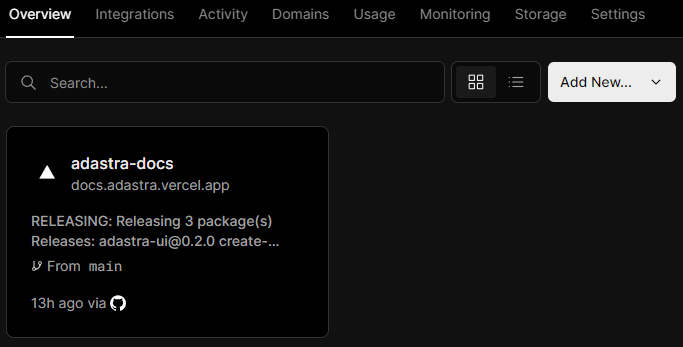
\includegraphics{images/vercelPanel.png}
    \caption{Panel principal de Vercel}
    \label{fig:vercelPanel}
\end{figure}

\begin{figure}
    \centering
    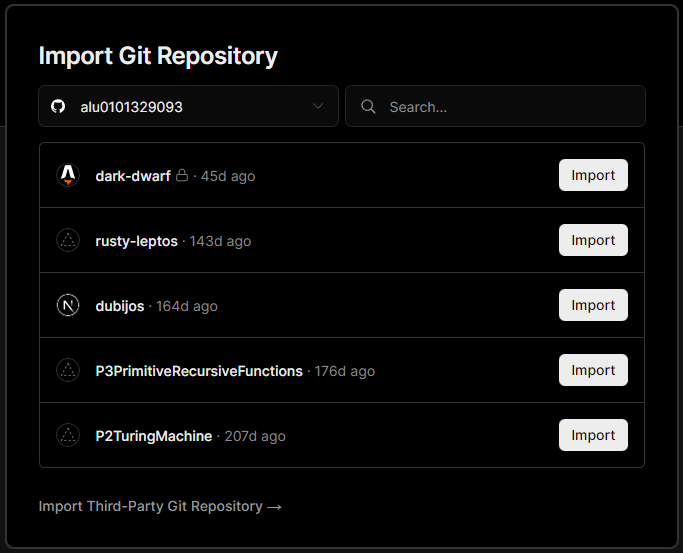
\includegraphics{images/vercelNewProject.png}
    \caption{Panel para añadir un nuevo proyecto en Vercel}
    \label{fig:vercelNewProject}
\end{figure}

\begin{figure}
    \centering
    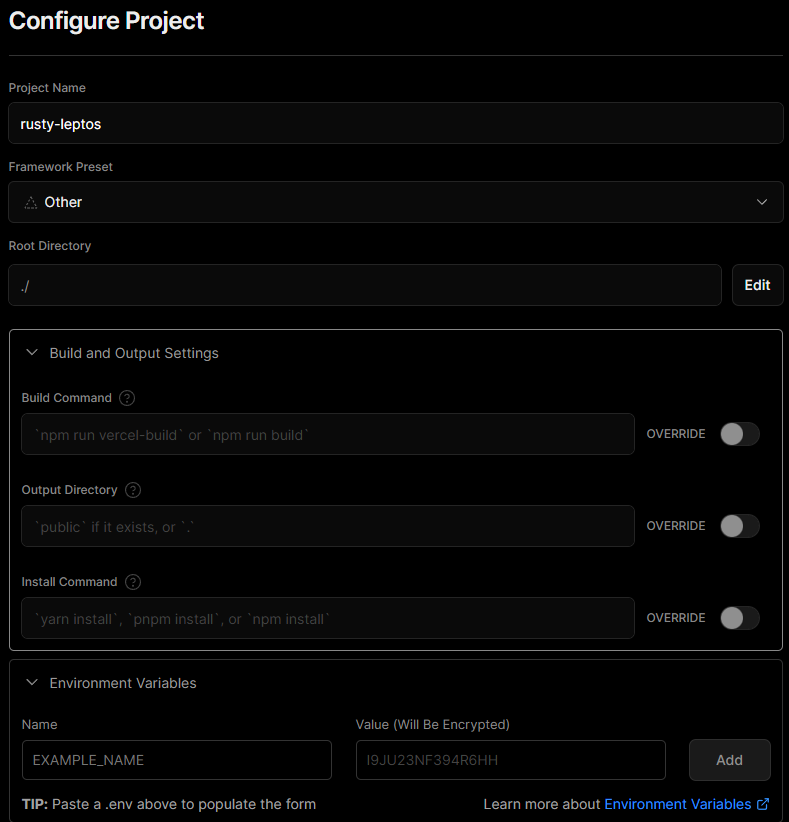
\includegraphics{images/vercelConfig.png}
    \caption{Panel de configuración del nuevo proyecto en Vercel}
    \label{fig:vercelConfig}
\end{figure}
%%%%%%%%%%%%%%%%%%%%%%%%%%%%%%%%%%%%%%%%%%%%%%%%%%%%%%%%%%%%%%%%%%%%%%%%%%%%%%%
\newpage{\pagestyle{empty}}
\thispagestyle{empty}

\chapter{\LARGE Diseño}
\label{chapter:tres}

En este capítulo se explica el porqué se han tomado ciertas decisiones, problemas y dudas que han ido surgiendo a lo largo del desarrollo y se muestra las especificaciones del sistema.

\section{Consideraciones de Diseño}
Cuando se utiliza GitHub en el ámbito académico no hay una sola forma de organizar las clases y queda a criterio de cada profesor. Es por esto que una aplicación inflexible no puede llegar muy lejos. Como resultado, se ha decidido crear una sistema generalista en el que permita al usuario modificar lo máximo posible el resultado final. Todo esto se puede realizar gracias a un archivo de configuración, el cual permite tanto modificar la apariencia de la aplicación como el propio contenido de esta.

El hecho de que ciertos apartados de la aplicación no estén en el ecosistema de GitHub llega a ser un gran problema, ya que no se pueden obtener por la API de GitHub, por esto se permite que los enlaces a esas secciones se puedan introducir a través de la configuración. Por lo que se permitirá cambiar cosas como el nombre de la aplicación y los enlaces a los diferentes contenidos como el google classroom o parecidos, campus virtual de la asignatura, etc.

Otro punto a destacar sería el hecho de que muchas veces un profesor puede querer relacionar ciertos contenidos como las clases, labs o temas entre ellos. Es por esto que para simplificar la experiencia del usuario se les permite introducir en el encabezado de los diferentes archivos markdown, las key de otros archivos para poner enlaces a ellos de manera automática en la página creada.

\section{El inicializador de {\tt adastra}}
Como punto de inicio para usar la aplicación se ha decidido seguir un patrón que siguen la gran mayoría de paquetes en el ámbito de desarrollo de aplicaciones con Javascript y npm. Este se basa en usar el comando \verb|create| de los manejadores de paquetes como npm o yarn. El comando de inicio de adastra sería el siguiente:

\begin{verbatim} pnpm create adastra-lms\end{verbatim}
Este comando buscará un paquete con el nombre \verb|create-{name}|, siendo el \verb|name| el parámetro que se le pase al comando, en este caso para adastra sería el paquete \verb|create-adastra-lms| y se ejecutaría para crear un proyecto la aplicación. Este sistema lo usan la mayoría de framework populares de JS como React o incluso Astro, el framework usado por esta aplicación.

\section{La template del proyecto}
Tras haber ejecutado el comando anterior se creará el proyecto en función de la template que se ha creado para este. Dentro de esta se ha dotado de muchas funcionalidades para simplificar y mejorar la experiencia del usuario.

\subsection{Creación de contenido por Markdown}
El sistema más fundamental sería la creación del contenido principal de la aplicación que en este caso se divide en tres carpetas (labs, classes y subjects), en las cuales se podrá añadir nuevos archivos de tipo markdown con el fin de añadir contenido al LMS.

En este caso el contenido de cada carpeta está pensado para que se use de la siguiente manera:
\begin{itemize}
    \item \textbf{labs}: Comprendería las tareas y laboratorios de la asignatura.
    \item \textbf{classes}: Aquí irían información sobre las clases impartidas. Normalmente separando el contenido en días.
    \item \textbf{subjects}: Por último serían la información relacionadas con los diferentes temaríos de la asignatura. Normalmente habrá una o más clases y labs relacionadas con un subject.
\end{itemize}

\subsection{El sistema de navegación en función de la rutas}
Uno de los sistemas que más fácilmente se puede ver es que a lo largo del proyecto es que a la izquierda de la web producidad se encontraría una barra de navegación que de forma automática.

\subsection{El fichero de Configuración {\tt adastra.config.mjs}} \label{diseño:data}
Uno de los puntos claves al crear está template fue buscar la mayor flexibilidad posible a la hora de poder modificar los contenidos por el usuario, pero sin complicar demasiado el proceso. Es por eso que en un punto se decidió crear un archivo de configuración en que poder especificar ciertos cambios sin tener que modificar el código directamente el usuario.

Dentro de este archivo se estableció dos posibles configuraciones que el usuario quería cambiar:
\begin{itemize}
    \item \textbf{tailwindConfig}: En esta sección se podrá añadir cambios a la propia configuración de la librería de estilos usada por la template para así poder modificar la apariencia de la aplicación de manera sencilla.
    \item \textbf{organizationInfo}: La última sección, pero no menos importante, serviría para añadir nueva información que la aplicación no pueda obtener de la API de GitHub o que se quiera que el usuario pueda decidir que añadir. Algunos ejemplos de esto sería el título que saldría en la aplicación o el link a el campus virtual de la asignatura.
\end{itemize}

En la figura \ref{fig:adastraConfig} se puede ver un ejemplo de la configuración.

%%%%%%%%%%%%%%%%%%%%%%%%%%%%%%%%%%%%%%%%%%%%%%%%%%%%%%%%%
\newpage{\pagestyle{empty}}
\thispagestyle{empty}

\chapter{\LARGE Implementación}
\label{chapter:cuatro}

El objetivo de este capítulo es demostrar las partes importantes o de interés de la implementación y como se ha logrado la realización de lo mencionado en capítulos anteriores.

\section{El monorepo del proyecto}

Una de las cosas fundamentales a la hora de crear este proyecto era conseguir dividir el proyecto en varias secciones sin dificultar el trabajar con ellas a la vez. Es por esto que se decidió usar un monorepo para guardar el proyecto y aprovechar de ciertas herramientas para facilitar su uso. Como herramienta principal para gestionar el monorepo se decidió usar \verb|turborepo|\cite{turborepo}, debido a que es uno de las más populares y de los que más rendimiento tienen a la hora de construir las aplicaciones. Además de usar turborepo, se decidió aprovechar una de las opciones que trae el gestor de paquetes \verb|pnpm|\cite{pnpm}, los \verb|worspaces|\cite{pnpm-workspaces}, la cual permite unir varios proyectos dentro del mismo repositorio y compartir las dependencias entre ellos. Por último, se utilizó la herramienta \verb|changesets|\cite{changesets} para el control de versiones de los diferentes paquetes y proyectos del monorepo.

\section{El inicializador de {\tt adastra}}

Como se dijo anteriormente en el apartado de diseño se ha creado un paquete llamado \verb|create-adastra-lms|, que sirve como punto de inicio para crear un proyecto con AdAstra. La función principal de este paquete se muestra en la figura \ref{fig:adastraCreateMain}. Lo primero que se realiza es la extracción de los argumentos pasados al programa, para luego crear un objeto \verb|context|, que proporciona los datos que necesitará la aplicación, en función de estos argumentos. En caso de que se haya pasado como argumento una \textit{flag} de ayuda, como \verb|-h| o \verb|--help|, se mostrará el menú de ayuda como resultado, se puede ver en la figura \ref{fig:adastraCreateHelp}. Para finalizar, se ejecutarán los diferentes pasos de la ejecución, encapsulados dentro de un array, que en este caso se tratan de diferentes funciones asíncronas que se llamarán una después de otra. Para facilitar el proceso de creación de este paquete se ha usado, una librería del framework de \verb|Astro|\cite{astro} llamada \verb|@astrojs/cli-kit|\cite{astro-cli} que suministra de diferentes utilidades que sirven para facilitar la creación de un programa de cli, como la petición de un prompt o las personalización de los mensajes. 

\begin{figure}
    \begin{lstlisting}[language=Javascript]
        export const main = async () => {
          const clearArgv = process.argv.slice(2).filter((arg) => arg !== "--");
          const context = getContext(clearArgv);
          if (context.help) return help();
        
          const steps = [projectName, template, dependecies, git, next];
        
          for (const step of steps) {
            await step(context);
          }
        
          exit();
        };
    \end{lstlisting}
    \caption{Función principal de create-adastra-lms}
    \label{fig:adastraCreateMain}
\end{figure}

\begin{figure}
    \centering
    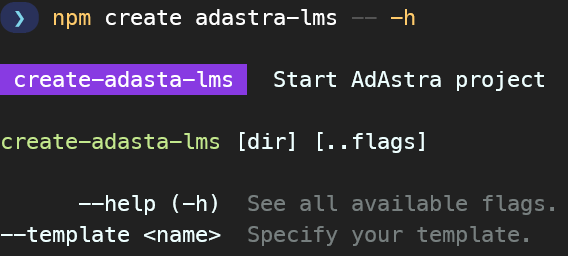
\includegraphics{images/adastraHelp.png}
    \caption{Salida del flag de ayuda de create-adastra-lms}
    \label{fig:adastraCreateHelp}
\end{figure}

Ahora vamos a explicar en más profundidad cada parte.

\subsection{La función {\tt getContext}}
Está función se encarga de extraer los valores de los argumentos y convertirlo a los datos deseados a través de la librería \verb|arg|\cite{arg}. Tras se usará el primer parametro pasado como \verb|cwd| y posible nombre del proyecto a crear y se usa la función \verb|detectPackageManager| de la librería \verb|which-pm-runs|\cite{which-pm-runs} para detectar cual manejador de paquetes se está usando y guardar este dato. Con todo esto se construirá un objeto \verb|context| que será el resultado de la función. En la figura \ref{fig:adastraCreateContext} se puede ver en más profundidad esta función.

\begin{figure}
    \begin{lstlisting}[language=Javascript]
        export interface Context {
          help: boolean;
          prompt: typeof prompt;
          cwd: string;
          pkgManager: string;
          projectName?: string;
          template?: string;
          install?: boolean;
          exit(code: number): never;
        }

        export const getContext = (argv: string[]): Context => {
          const flags = arg(
            {
              "--help": Boolean,
              "--template": String,
        
              "-h": "--help",
            },
            { argv, permissive: true }
          );
        
          const pkgManager = detectPackageManager()?.name ?? "npm";
          let cwd = flags["_"][0];
          let { "--help": help = false, "--template": template } = flags;
          let projectName = cwd;
        
          const context: Context = {
            help,
            prompt,
            pkgManager,
            projectName,
            template,
            cwd,
            exit: (code) => {
              process.exit(code);
            },
          };
          return context;
        };
    \end{lstlisting}
    \caption{Función getContext de create-adastra-lms}
    \label{fig:adastraCreateContext}
\end{figure}

\subsection{El paso {\tt projectName}}

Dentro de este paso lo primero que se comprueba es que en caso de si se ha pasado un \verb|cwd| como argumento, este sea valido para usar y este vació. En caso de que la comprobación sea fallida, el programa pedirá al usuario que la ubicación deseada a usar, comprobando que esta sea valida, esta ubicación será el cwd a usar para el proyecto. Tras esto, tanto si el cwd fue valido o no, se extraerá un nombre valido para el proyecto, con la función \verb|toValidName|, que corrigue a un nombre valido el string que se le pase. En la figura \ref{fig:adastraCreateProjectName} se ve las partes importantes del código de este paso.

\begin{figure}
    \begin{lstlisting}[language=Javascript]
        const checkCwd = async (cwd: string | undefined) => {
          const empty = cwd && isEmpty(cwd);
          if (empty) {
            log("");
            await info(
              "dir",
              `Using ${color.reset(cwd)}${color.dim(" as project directory")}`
            );
          }
        
          return empty;
        };
        
        export const projectName = async (context: Context) => {
          await checkCwd(context.cwd);
        
          if (!context.cwd || !isEmpty(context.cwd)) {
            if (!isEmpty(context.cwd)) {
              await info(
                "Hmm...",
                `${color.reset(`"${context.cwd}"`)}${color.dim(` is not empty!`)}`
              );
            }
        
            const { name } = await context.prompt({
              name: "name",
              type: "text",
              label: title("dir"),
              message: "Where should we create your new project?",
              initial: `./${generateProjectName()}`,
            });
        
            context.cwd = name!;
            context.projectName = toValidName(name!);
          } else {
            let name = context.cwd;
            context.projectName = toValidName(extractName(name));
          }
        
        };
    \end{lstlisting}
    \caption{Paso projectName de create-adastra-lms}
    \label{fig:adastraCreateProjectName}
\end{figure}

\subsection{El paso {\tt template}}

Este es uno de los pasos más importantes y es que este se encarga de descargar y preparar la \textit{template}, de la cual hablaremos después, a usar para el proyecto. Lo primero que se hace es comprobar si se ha pasado una template como argumento, en caso negativo, se le pide al usuario de entre una lista de templates que escoja la deseada. Tras saber que template se va a querer usar, se empezará el proceso de copia de esta en el que se llamará a la función \verb|copyTemplate| En la figura \ref{fig:adastraCreateTemplate} se puede el código de este paso. Dentro de esta primero se intentará descargar la template deseada con la librería \verb|giget|\cite{giget}, que facilita la descarga de proyectos de GitHub a través de un programa de Javascript, a una carpeta llamada \verb|.adastra|, que guardara toda la lógica y funcionamiento del LMS. En caso de que la descarga de un error el programa se parará y mostrará el error. Si todo va bien lo siguiente que se hará es mover el archivo \verb|package.json| que trae la template, que en este caso esta dentro de \verb|.adastra/package.json| a la carpeta principal del proyecto para usarlo como el archivo \verb|package.json| de este proyecto. Tras haber reubicado este archivo se pasará a realizar ciertos cambios a este como cambiar el nombre al del proyecto y cambiar los \verb|scripts| de npm para que seán los siguientes:
\begin{verbatim}
    scripts: {
        dev: 'astro dev --root "./.adastra"',
        build: 'astro build --root "./.adastra"',
    }
\end{verbatim}
Con estos scripts se define que se deberá usar la carpeta \verb|.adastra| como la carpeta principal a usar por el framework Astro, esto se debe a que para simplificar la experiencia del usuario se decide ocultar la lógica principal del programa de Astro creado en la carpeta \verb|.adastra|, por lo que se deberá usar esa carpeta como \verb|root| del proyecto y no la carpeta principal como normalmente haría el framework. Tras esto se moverá también el archivo \verb|.gitignore| de la template a la carpeta principal, se creará el archivo .env  para que el usuario pueda introducir la variable de entorno \verb|GITHUB_SECRET| en local y el archivo \verb|adastra.config.mjs| con la configuración necesaria del proyecto. Por último se crearán link simbólicos que permitan modificar el contenido del proyecto de Astro dentro de \verb|.adastra|, pero sin tener que entrar dentro de la lógica de este. Estos serían los siguientes:

\begin{itemize}
    \item Se vinculará el archivo \verb|.env| creado en la carpeta principal del proyecto con uno dentro de la carpeta \verb|.adastra|, esto es necesario ya que al definir anteriormente que el root a usar a la hora de iniciar el framework de astro fuera la carpeta \verb|.adastra| de normal mirará ahi si se encuentra el archivo \verb|.env| y no fuera de esta.
    \item Se vinculará las carpetas \verb|classes|, \verb|labs| y \verb|subjects| con las carpetas con sus respectivas contra partes dentro de la carpeta \verb|content| del proyecto de Astro, donde se guarda los contenido markdown a usar. En este caso serían:
    \begin{verbatim}
        .adastra/src/content/docs/1-activities/1-classes
        .adastra/src/content/docs/1-activities/2-labs
        .adastra/src/content/docs/1-activities/3-subjects
    \end{verbatim}
\end{itemize}

En la figura \ref{fig:adastraCreateTemplateCopy} se puede ver mejor la función \verb|copyTemplate|.

\begin{figure}
    \begin{lstlisting}[language=Javascript]
        export const template = async (context: Context) => {
          if (!context.template) {
            const { template: tmpl } = await context.prompt({
              name: "template",
              type: "select",
              label: title("tmpl"),
              message: "How would you like to start your new project?",
              initial: "basic",
              choices: [
                {
                  value: "basic",
                  label: "Basic LMS",
                  hint: "(recommended)",
                },
              ],
            });
            context.template = tmpl;
          } else {
            await info(
              "tmpl",
              `Using ${color.reset(context.template)}${color.dim(
                " as project template"
              )}`
            );
          }
        
          await spinner({
            start: "Template copying...",
            end: "Template copied",
            while: () =>
              copyTemplate(context.template!, context as Context).catch((e) => {
                if (e instanceof Error) {
                  error("error", e.message);
                  process.exit(1);
                } else {
                  error("error", "Unable to clone template.");
                  process.exit(1);
                }
              }),
          });
        };
    \end{lstlisting}
    \caption{Paso template de create-adastra-lms}
    \label{fig:adastraCreateTemplate}
\end{figure}

\begin{figure}
    \begin{lstlisting}[language=Javascript]
        const copyTemplate = async (template: string, context: Context) => {
          const templateTarget = `.../${template}`;
        
          try {
            await downloadTemplate(templateTarget, {
              force: true, provider: "github", cwd: context.cwd, dir: "./.adastra"
            });
          } catch (err: any) {
            throw new Error(err.message);
          }
        
          fs.renameSync(`${context.cwd}/.adastra/package.json`,`${context.cwd}/package.json`);
        
          const updateFiles = Object.entries(FILES_TO_UPDATE).map(
            async ([file, update]) => {
              const fileLoc = path.resolve(path.join(context.cwd, file));
              if (fs.existsSync(fileLoc)) {
                return update(fileLoc, {
                  name: context.projectName!,
                  scripts: {
                    dev: 'astro dev --root "./.adastra"',
                    build: 'astro build --root "./.adastra"',
                  },
                });
              }
            }
          );
        
          await Promise.all([...updateFiles]);
        
          fs.renameSync(`${context.cwd}/.adastra/.gitignore`,`${context.cwd}/.gitignore`);
          fs.writeFileSync(`${context.cwd}/.env`, "GITHUB_SECRET=\n");
        
          fs.writeFileSync(
            `${context.cwd}/adastra.config.mjs`,
            `export const tailwindConfig = { ... };
        
        export const organizationInfo = { ... };
        `);
        
          fs.symlinkSync(`../.env`, `${context.cwd}/.adastra/.env`, "file");
          symlinkDir(`${context.cwd}/.adastra/public`, `${context.cwd}/public`);
          symlinkDir(`${context.cwd}/.adastra/src/content/docs/1-activities/1-classes`,`${context.cwd}/classes`);
          ...
        };
    \end{lstlisting}
    \caption{Función copyTemplate simplificada del paso template de create-adastra-lms}
    \label{fig:adastraCreateTemplateCopy}
\end{figure}

\subsection{El paso {\tt dependencies}}

En el siguiente paso de la ejecución se le preguntará al usuario si se querrá instalar las dependencias ahora, sino se le notificará que deberá hacerlo más tarde. Si se acepta instalar, el programa usará la librería \verb|execa|\cite{execa}, que facilita la ejecución de otros procesos, para llamar el comando \verb|install| junto con el manejador de paquetes, que anteriormente se había detectado y guardado en \verb|context|. En la figura \ref{fig:adastraCreateDependencies} se puede ver el codigo de esto.

\begin{figure}
    \begin{lstlisting}[language=Javascript]
        const install = async ({
          pkgManager,
          cwd,
        }: {
          pkgManager: string;
          cwd: string;
        }) => {
          const installExec = execa(pkgManager, ["install"], { cwd });
          return new Promise<void>((resolve, reject) => {
            setTimeout(() => reject(`Request timed out after one minute`), 300_000);
            installExec.on("error", (e) => reject(e));
            installExec.on("close", () => resolve());
          });
        };
        
        export const dependecies = async (context: Context) => {
          const { deps } = await context.prompt({
            name: "deps",
            type: "confirm",
            label: title("deps"),
            message: `Install dependencies?`,
            hint: "recommended",
            initial: true,
          });
          context.install = deps;
        
          if (!deps)
            return await info(
              "No problem!",
              "Remember to install dependencies after setup."
            );
        
          await spinner({
            start: `Dependencies installing with ${context.pkgManager}...`,
            end: "Dependencies installed",
            while: () =>
              install({ pkgManager: context.pkgManager, cwd: context.cwd }).catch(
                (e) => {
                  error("error", e);
                  process.exit(1);
                }
              ),
          });
        };
    \end{lstlisting}
    \caption{Paso dependencies de create-adastra-lms}
    \label{fig:adastraCreateDependencies}
\end{figure}

\subsection{El paso {\tt git}}

Este paso es parecido al anterior, solo que en este caso se pregunta si se quiere iniciar un proyecto de \verb|git|\cite{git}, en caso de que no existiera previamente. En caso afirmativo, se usará \verb|execa| al igual que antes para llamar en este caso los siguientes comandos de git que permiten empezar un repositorio:
\begin{verbatim}
    git init
    git add -A
    git commit -m Initial commit from AdAstra 
\end{verbatim}

En la figura \ref{fig:adastraCreateGit} se puede visualizar el código de este paso.

\begin{figure}
    \begin{lstlisting}[language=Javascript]
        const init = async ({ cwd }: { cwd: string }) => {
          try {
            await execa("git", ["init"], { cwd, stdio: "ignore" });
            await execa("git", ["add", "-A"], { cwd, stdio: "ignore" });
            await execa(
              "git",
              [
                "commit",
                "-m",
                "Initial commit from AdAstra",
              ],
              { cwd, stdio: "ignore" }
            );
          } catch (e) {
            console.error(e)
          }
        };
        
        export const git = async (context: Context) => {
          if (fs.existsSync(path.join(context.cwd, ".git")))
            return await info("Nice!", `Git has already been initialized`);
        
          const { git } = await context.prompt({
            name: "git",
            type: "confirm",
            label: title("git"),
            message: `Initialize a new git repository?`,
            hint: "optional",
            initial: true,
          });
        
          if (!git)
            return await info(
              "Sounds good!",
              `You can always run ${color.reset("git init")}${color.dim(" manually.")}`
            );
        
          await spinner({
            start: "Git initializing...",
            end: "Git initialized",
            while: () =>
              init({ cwd: context.cwd }).catch((e) => {
                error("error", e);
                process.exit(1);
              }),
          });
        };
    \end{lstlisting}
    \caption{Paso git de create-adastra-lms}
    \label{fig:adastraCreateGit}
\end{figure}




% \begin{figure}[H]
%     \centering
%     \makebox[\textwidth][c]{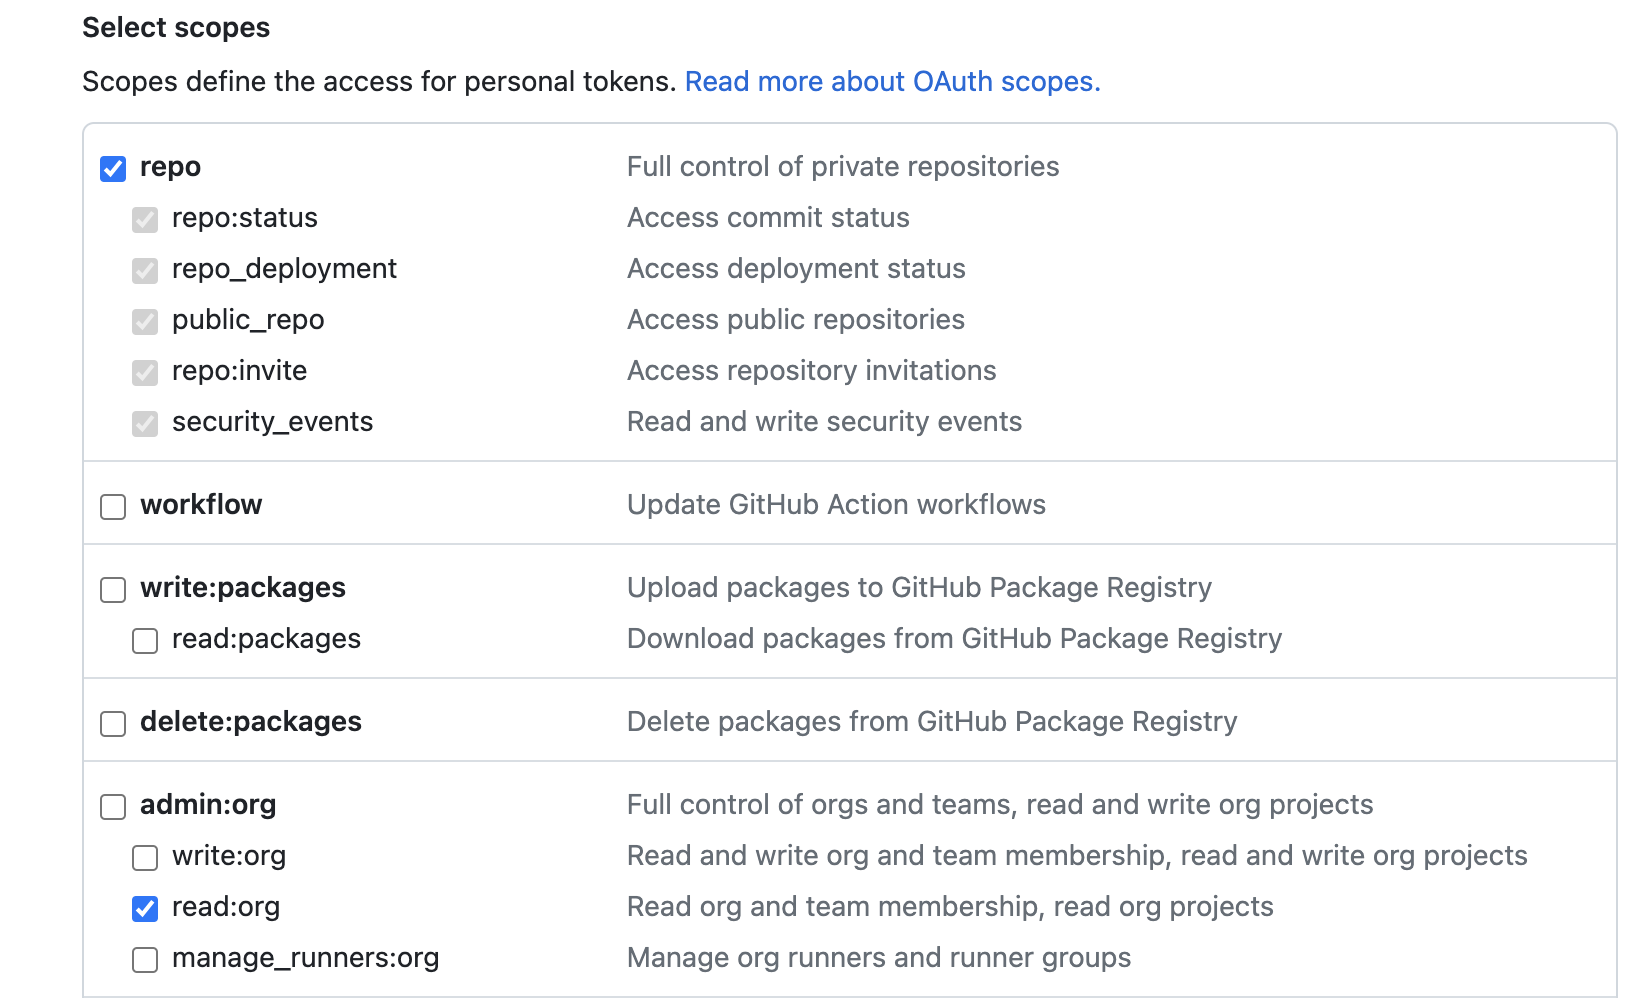
\includegraphics[width=\textwidth]{images/scopes.png}}
%     \caption{Scopes para el token GITHUB\_SECRET}
%     \label{fig:scopes}
% \end{figure}


% \section{El controlador}
% Como se ha comentado en capítulos anteriores, la mayoría de comandos se aprovecha de los comandos ya proporcionados por \verb|gh|. Como es el caso de \verb|gh edu install|. Después de determinar si la extensión es \emph{first-party} o \emph{third-party} (extensión independiente de la organización \verb|gh-cli-for-education|), se obtiene la dirección del repositorio de la extensión, se invoca \verb|gh extension install| y se añade a \verb|data.json|.

% \begin{figure}[H]
%     \centering
%     \makebox[\textwidth][c]{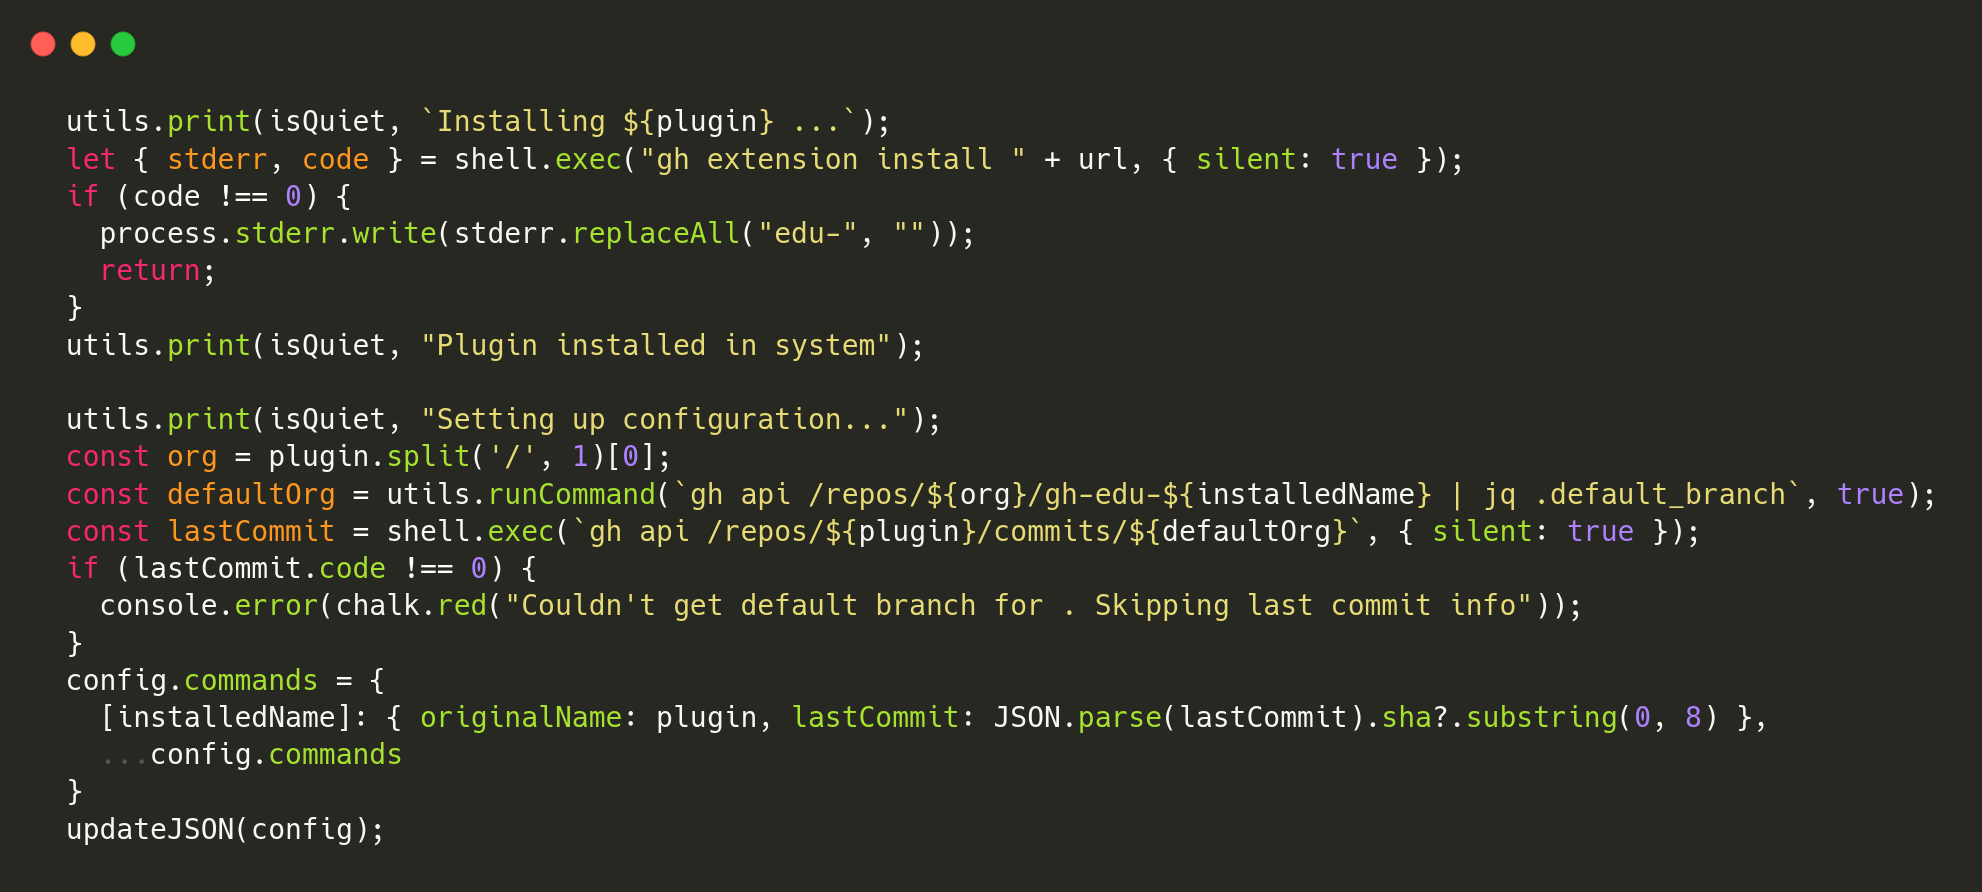
\includegraphics[width=\textwidth]{images/installCode.png}}
%     \caption{Implementación. Código para instalar extensiones}
%     \label{fig:installCode}
% \end{figure}

% En la figura \ref{fig:installCode} vemos que después de instalar la extensión, hacemos una llamada \emph{API REST} para saber cuál es la rama por defecto. Al tener esta información, podemos buscar cuál es el \gls{hash} del último \emph{commit}, para actualizar el campo \verb|lastCommit|.

% \emph{Nota: utils.print() es una función muy simple para determinar si el mensaje debería imprimirse o no, dependiendo del valor del flag --quiet}.

% Para que \verb|commander| acepte únicamente las extensiones instaladas, se ha escrito el siguiente código (figura \ref{fig:addThirdParty}):

% \begin{figure}[H]
%     \centering
%     \makebox[\textwidth][c]{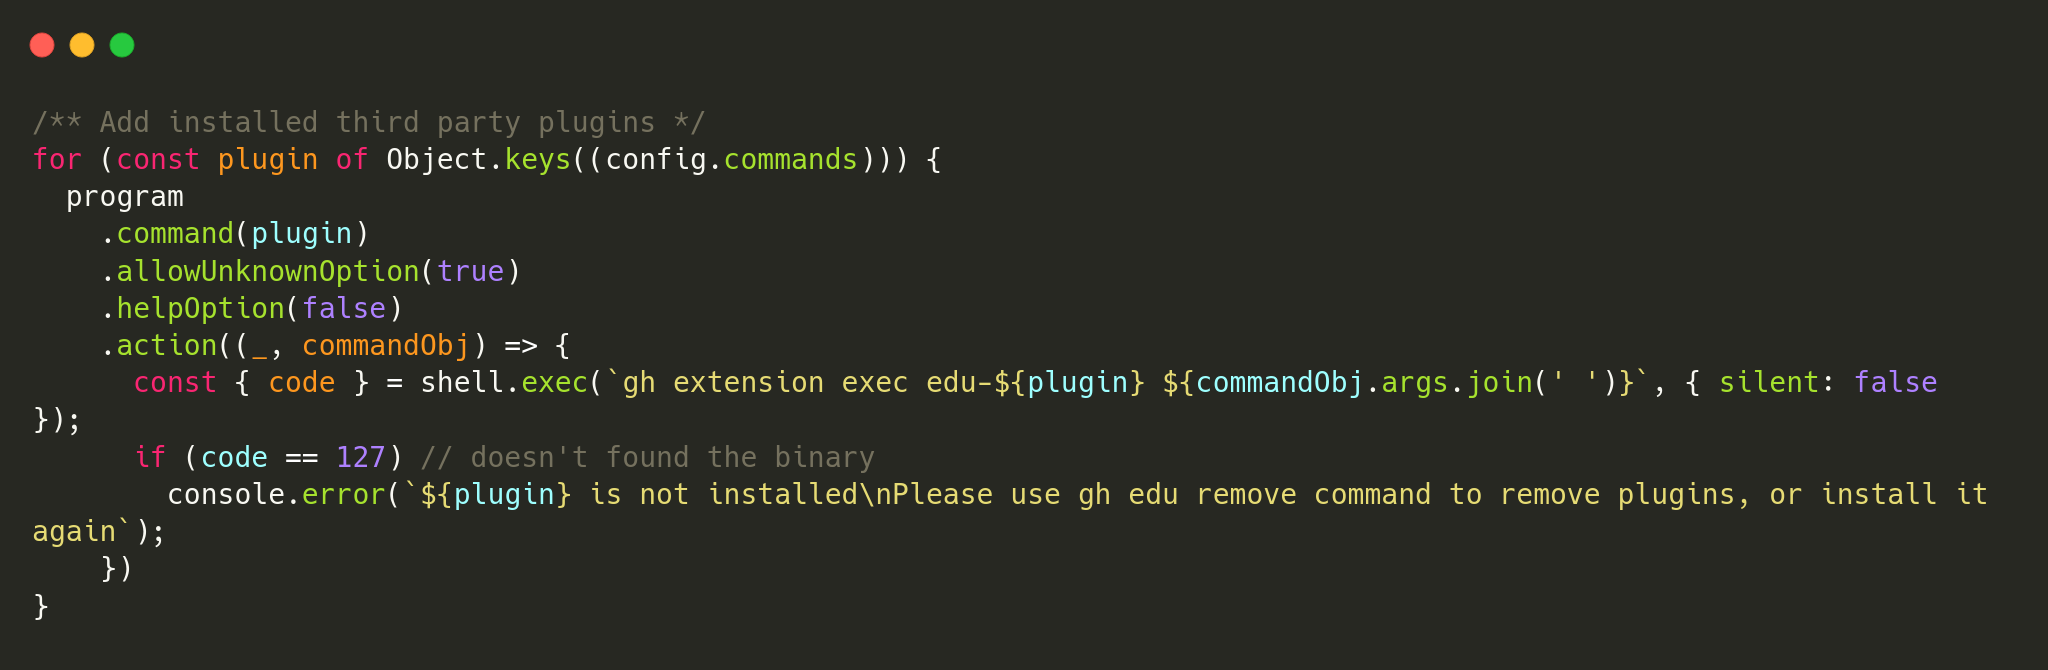
\includegraphics[width=\textwidth]{images/addThirdParty.png}}
%     \caption{Implementación. Controlador. Añadir extensiones third-party}
%     \label{fig:addThirdParty}
% \end{figure}

% Todas las extensiones, que se hayan instalado en el sistema a través de \verb|gh-edu|, se añadirán como comandos disponibles. También se activa la posibilidad de usar opciones desconocidas y se delega su gestión al subcomando en cuestión. Así mismo se desactiva la ayuda y en el manejo de errores solo se comprueba que el comando haya sido ejecutado, pues naturalmente de estas tareas se tiene que ocupar cada extensión.

% Aquí se deja ver la madurez del programa al permitirnos utilizar comandos desconocidos, función que, al momento de escribir estas líneas, todavía no es posible con \href{https://github.com/spf13/cobra/issues/739}{cobra}.

% \subsection{Manejo del único punto de información: data.json} \label{impl:data.json}
% Lo primero que el programa hace al ser ejecutado, es comprobar la validez del fichero. La siguiente figura (\ref{fig:dataGraph}) muestra los estados por los que se pasa para lograrlo.

% \begin{figure}[H]
%     \centering
%     \makebox[\textwidth][c]{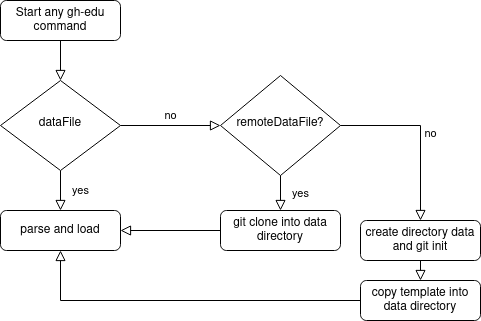
\includegraphics[width=0.5\textwidth]{images/createConfig.png}}
%     \caption{Obtención del archivo data.json}
%     \label{fig:dataGraph}
% \end{figure}

% Es primer paso es comprobar si se encuentra en la localización correspondiente (\verb|~/.config/gh-edu/data.json|). De no ser así, se intenta conseguirlo desde el repositorio \verb|gh-edu-profile|. Como última instancia se crea un fichero nuevo, partiendo de una plantilla que contiene todos los campos necesarios.

% Sabiendo que el fichero está disponible, pasamos a validar su contenido. Primero se \glspl{deserialization} para comprobar que es un fichero JSON válido. Acto seguido pasamos a realizar una comprobación simple de los campos, comprobando que estén en el fichero y que las \glspl{regex} sean válidas.

% \begin{figure}[H]
%     \centering
%     \makebox[\textwidth][c]{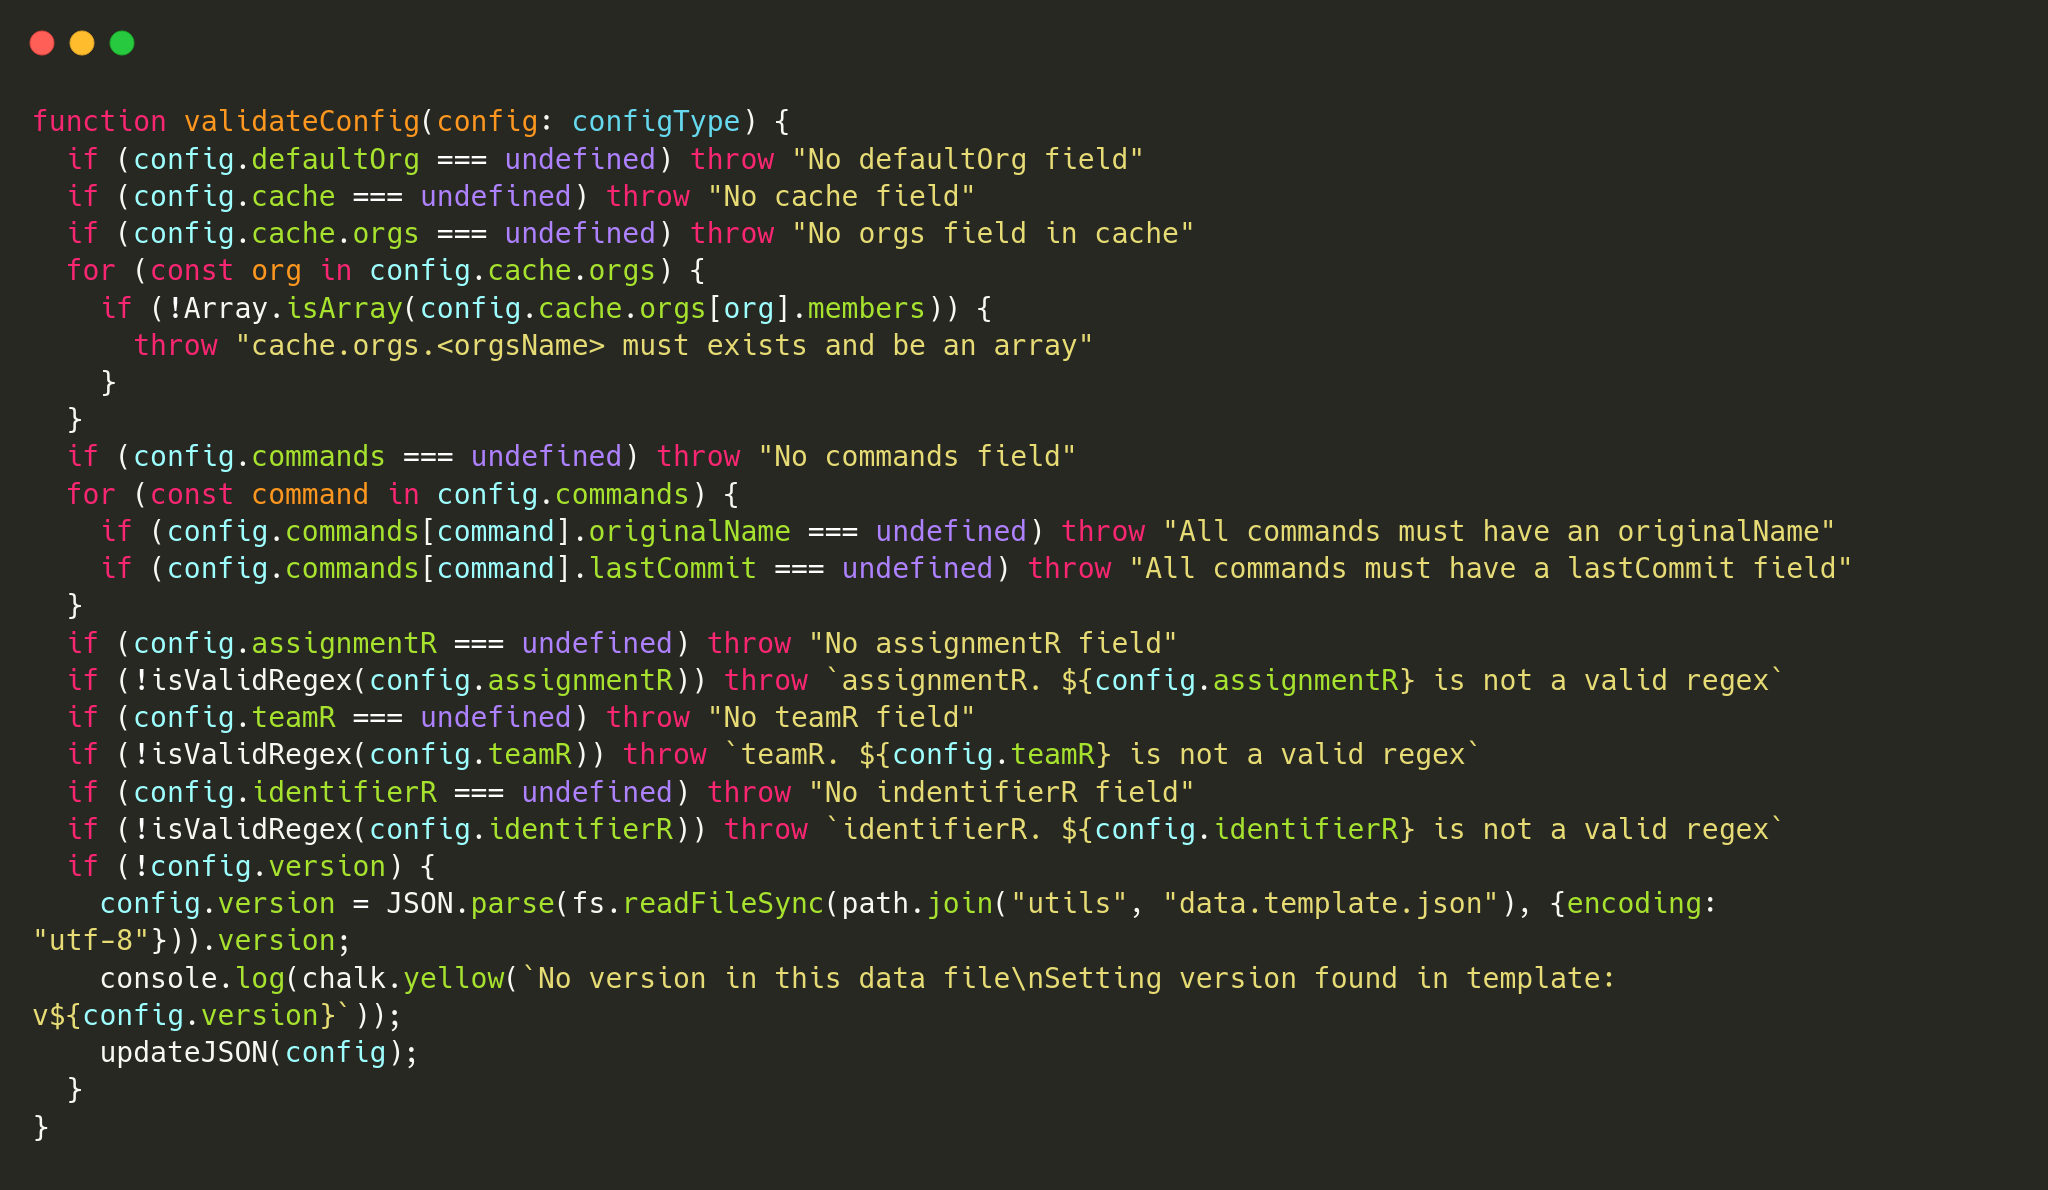
\includegraphics[width=\textwidth]{images/comprobacion.png}}
%     \caption{Implementación. data.json. Comprobamos que los campos son válidos}
%     \label{fig:comprobar}
% \end{figure}

% Cada vez que se quiera actualizar la información, se actualiza la variable donde se cargó el fichero, se \glspl{serialization} y se escribe de vuelta al fichero.

% \section{Extensión minimalista: {\tt gh-edu-view}}\label{sec:gh-edu-view-implementation}

% A la hora de escribir una extensión para \verb|gh-edu| en \verb|JS|, se procede de la misma forma que con una extensión \verb|gh|.
% Deben crearse los ficheros \verb|gh-edu-view/gh-edu-view| (script bash) y \verb|gh-edu-view/gh-edu-view.js| (programa \verb|JS|).

% Para intentar conseguir los identificadores relacionados a los alumnos, con nada más que la información proporcionada con GitHub, no nos queda otra opción que buscar en todos los campos, donde dicha información podría estar disponible, y devolver un \emph{array} con todos los posibles resultados.

% \begin{figure}[H]
%     \centering
%     \makebox[\textwidth][c]{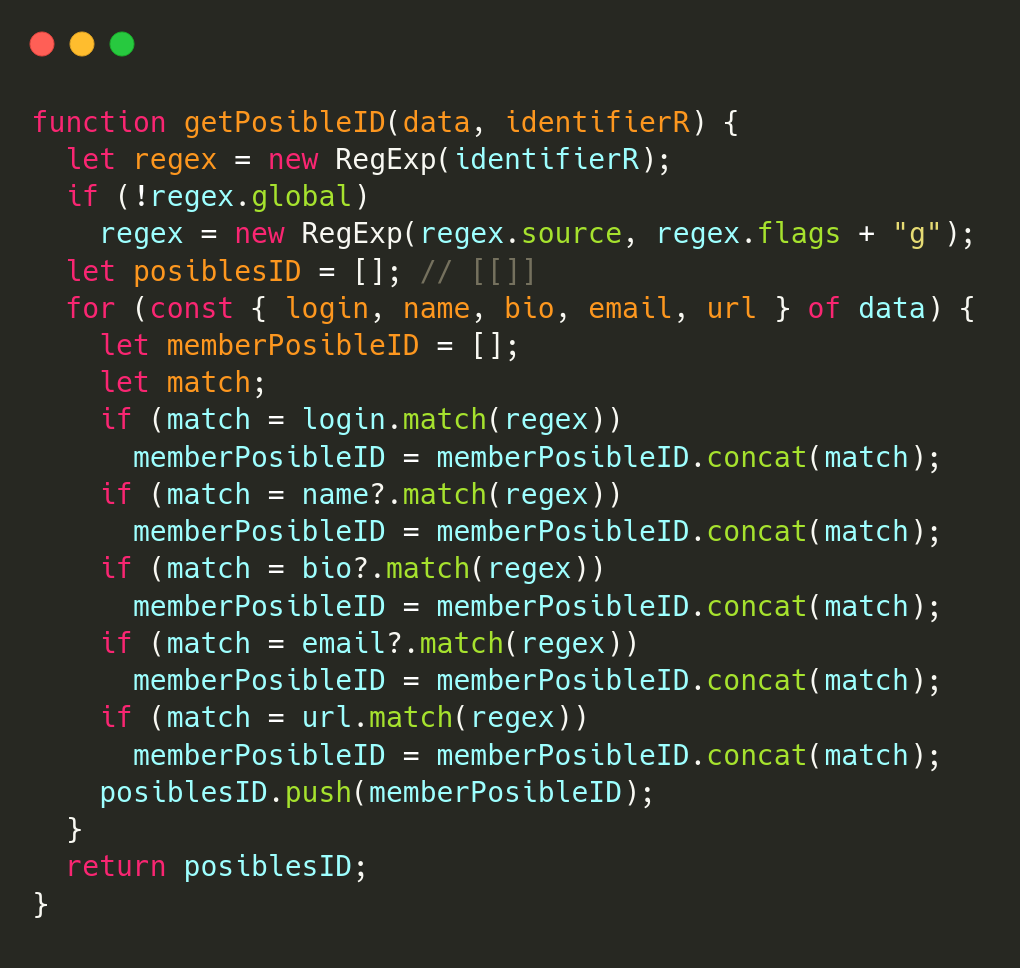
\includegraphics[width=0.5\textwidth]{images/posibleID.png}}
%     \caption{Implementación. gh-edu-view. Obtención de posibles identificadores}
%     \label{fig:viewId}
% \end{figure}

% Toda la información proporcionada por el comando \verb|members| se puede conseguir con una simple petición en GraphQL (figura \ref{fig:viewQuery}).

% \begin{figure}[H]
%     \centering
%     \makebox[\textwidth][c]{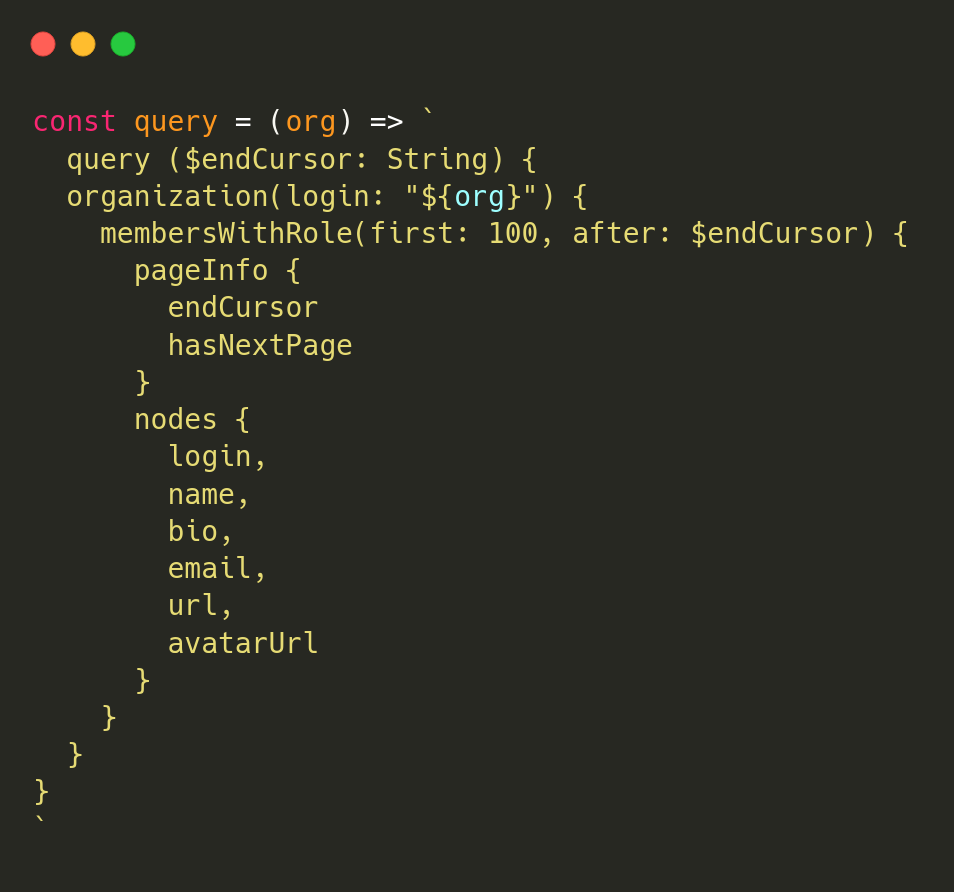
\includegraphics[width=0.5\textwidth]{images/view-query.png}}
%     \caption{Implementación. gh-edu-view. Petición para conseguir diversos campos de cada alumno}
%     \label{fig:viewQuery}
% \end{figure}

% \section{{La librería \tt shelljs} y el manejo de E/S: {\tt gh-edu-data}} \label{impl:gh-edu-data}
% Uno de los defectos de \verb|shelljs| que ya se ha comentado en el apartado de \textbf{Tecnologías} (\ref{shelljs}) es como no permite el uso de \verb|STDIN| o tuberías. Algo importante en este proyecto, pero especialmente en esta extensión por el uso avanzado de \verb|fzf| y \verb|jq|. Estas dos tecnologías, a pesar de ser completamente independientes la una a la otra, pueden trabajar conjuntamente gracias a su diseño flexible y minimalista a través de tuberías, haciendo posible la previsualización dinámica de los elementos en el comando \verb|log| (figura \ref{fig:interface-log})

% Este comportamiento es requerido, ya que no es posible pasar un objeto \verb|JS| o un \emph{array} al input de un programa que todavía no ha sido ejecutado. Solo se puede usar cadenas de texto. Lo ideal es ejecutar el comando, y de forma asíncrona ir procesando la estructura de datos, enviando cadenas de texto, como se hace en \verb|gh-edu-plagiarism| (gracias a \href{https://pkg.go.dev/os/exec@go1.18.3#Cmd.StdinPipe}{cmd.StdInPipe}).

% Hasta que la \href{https://github.com/shelljs/shelljs/issues/424}{incidencia 424} no sea resuelta, se ha tenido que realizar una solución alternativa utilizando ficheros temporales. La idea consiste en formatear el objeto o \verb|array| y escribir el resultado en un fichero, de esta forma podemos leer el fichero y transmitir esa información por medio de una tubería a otro comando en el mismo momento en el que se ejecuta el comando.

% \section{Concurrencia con Go y CSP: {\tt gh-edu-plagiarism}} \label{diseño:gh-edu-plagiarism}
% A diferencia del resto de extensiones \verb|plagiarism| está implementado en Go. Uno de los motivos del cambio de lenguaje es demostrar como se puede desarrollar extensiones en cualquier lenguaje sin muchas dificultades.

% También, como se comentó en \textbf{Tecnologías} (\ref{go}) este programa es altamente concurrente y paralelo. Go cuenta con un modelo de concurrencia bastante particular basado en el trabajo teórico de Tony Hoare \emph{Communicating Sequential processes} (CSP) \cite{hoare1985communicating}.

% Para entender las explicaciones de esta sección es necesario conocer dos conceptos: las gorutinas y los canales. Las gorutinas son \glspl{corrutine} independientes que se ejecutan en hilos verdes (\emph{green threads}), los cuales son hilos emulados generados en tiempo de ejecución, estos hilos se multiplexan a hilos reales del procesador a través del \verb|Go scheduler|, que determina cuanto tiempo debe estar cada hilo verde consumiendo CPU.

% Los canales son la estructura de datos que nos permite enviar información de una gorutina a otra y también sirven de elemento sincronizador, cuando se envía un elemento, la gorutina no continua hasta que el otro lado (el emisor) haya recibido la información y viceversa.

% La explicación de la figura \ref{fig:plagiarism} en términos de código sería la siguiente:\\
% Cada bloque dentro del módulo \verb|Concurrent| es una gorutina que se ejecuta de forma independiente y cada flecha pertenece a un canal, que sincroniza y a su vez transmite información de una gorutina a otra.

% La gorutina \verb|clone| va creando a su vez gorutinas a medida que más repositorios se vayan filtrando. Debido a que las gorutinas apenas consumen recursos, está bien eliminar y crear tantas como queramos. No obstante, como estamos realizando programación paralela, tenemos que tener cuidado de que no haya muchas más gorutinas corriendo que núcleos disponibles en el procesador, pues entonces conseguiríamos el efecto contrario al deseado, ralentizando toda la aplicación debido al constante cambio de contexto entre hilos. Para limitar la creación de gorutinas al número de núcleos disponibles se ha utilizado un semáforo. Un semáforo es una variable o estructura de datos que permite una cantidad arbitraria de procesos. Un semáforo binario es a efectos prácticos un \verb|lock| o \verb|mutex|.

% \begin{figure}[H]
%     \centering
%     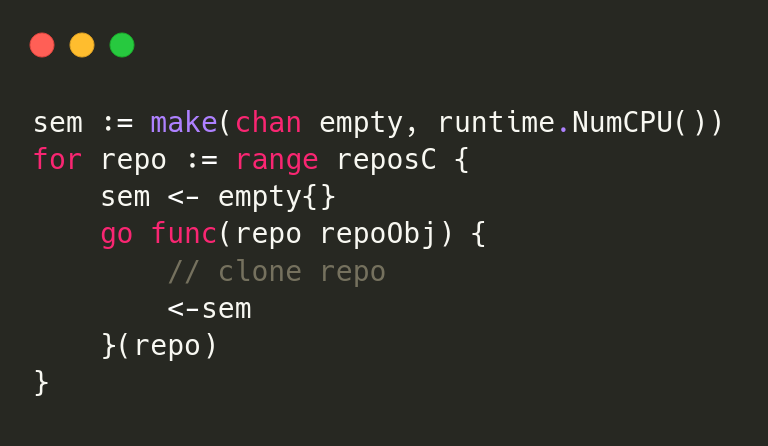
\includegraphics[width=0.5\linewidth]{images/concurrency-go.png}
%     \caption{Paralelismo limitado con un sémaforo}
%     \label{fig:concurrencyGo}
% \end{figure}
% El código que lo implementa (figura \ref{fig:concurrencyGo}) ha sido simplificado para explicar el funcionamiento del paralelismo y el semáforo.

% El canal \verb|sem| es un canal con buffer, esto quiere decir que no para el flujo (no sincroniza) hasta que el buffer se llene. El tamaño de dicho buffer es \verb|runtime.NumCPU()| que retorna el número de núcleos disponibles al ejecutar el programa. En cada iteración del bucle \verb|repo| contiene un nuevo repositorio proveniente del módulo \verb|Filter| y enviamos un elemento al canal \verb|sem|, el elemento en cuestión es irrelevante, estamos usando el canal por sus propiedades de sincronización, no para la transferencia de datos. Después ejecutamos una gorutina anónima que se encarga de clonar el repositorio, cuando termine escucha y descarta del canal \verb|sem|.

% De esta forma, si \verb|sem| está lleno significa que ya hay tantos procesos ejecutándose como núcleos hay disponibles, por lo que el programa queda en espera hasta que quede un hueco en el semáforo.

% % Esto va en diseño. Otro de los motivos por los cuales se eligió Go es que a la hora de diseñar la extensión me percate de que el programa sería altamente concurrente y paralelo. Uno de los motivos por los cuales se creó Go fue para poder aprovechar al máximo los varios núcleos que suele tener cualquier dispositivo moderno. Así, las instituciones educativas que reutilizan la misma organización para una misma asignatura a lo largo de varios años, y por ende tienen muchos repositorios y miembros, no verán su experiencia lastrada. También se tuvo en cuenta que Go tiene soporte de primera clase con \verb|gh| y uno de los casos de uso más comunes del lenguaje son aplicaciones CLI.

% \begin{figure}[H]
%     \centering
%     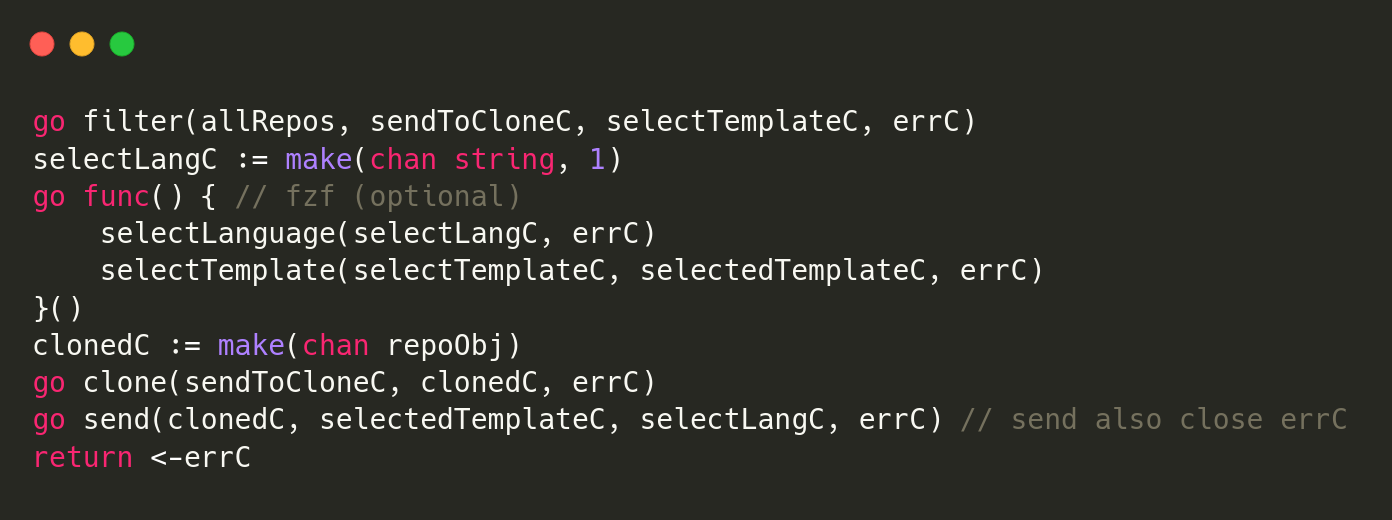
\includegraphics[width=\linewidth]{images/go-code.png}
%     \caption{Código general de plagiarism}
%     \label{fig:goCode}
% \end{figure}

 

%%%%%%%%%%%%%%%%%%%%%%%%%%%%%%%%%%%%%%%%%%%%%%%%%%%%%%%%%
\newpage{\pagestyle{empty}}
\thispagestyle{empty}

\chapter{\LARGE Conclusiones y líneas futuras}
\label{chapter:Resultados}

Lo que más resalto en este trabajo de fin de grado ha sido la tarea de diseñar una aplicación que sea generalista y fácil de usar para el usuario, pero sin perder la potencia y personalización que ofrecería crear un página web desde cero por el usuario. Es por esto, que siempre que se diseñaba nuevo contenido para el LMS nos preguntábamos si no rompía con la filosofía de que la experiencia de usuario siempre sea buena, y en caso de que no fuera así, aunque fuera algo muy potente, se dejaba de lado para siempre pensar en el usuario. Un ejemplo de ello fue el intentar añadir un sistema para autenticarse en el LMS, pero este sistema tenía la pega de que complicaría mucho lo que tendría que configurar el usuario, por esto aunque la idea era buena y estaba casi terminada se dio marcha atrás. \\
Aunque gran parte del trabajo ha sido cuesta arriba debido a las diferentes dificultades que encontramos por el camino de crear un LMS que fuera lo mejor posible, al final se consiguió crear un sistema que aunque pueda parecer simple a primera vista, siempre se le da la oportunidad al usuario de controlar casi al 100\% el resultado deseado. \\
Esto junto al hecho de que aprendí un gran numero de tecnologías, de las que antes no sabía nada o muy poco ha hecho que realmente el trabajo y esfuerzo halla valido la pena. Hay veces que incluso nos dejamos llevar por intentar siempre probar cosas nuevas que llego un punto en el que se tuvo que poner un límite, porque aunque la experiencia de aprender algo nuevo es muy bonita, al final este trabajo tenía una fecha final con la que cumplir, aun así las experiencias finales que me llevo me ayudarán en mi futuro y eso lo agradezco.
El trabajo de fin de grado está terminado, pero el proyecto puede crecer tanto como desee. Este tipo de proyecto requiere de trabajo constante y prolongado para que tenga acogida en los usuarios. Mis intenciones son seguir en algún momento contribuyendo a este proyecto y tomarlo como un proyecto personal.

%%%%%%%%%%%%%%%%%%%%%%%%%%%%%%%%%%%%%%%%%%%%%%%%%%%%%%%%%
\newpage{\pagestyle{empty}}
\thispagestyle{empty}

\chapter{\LARGE Summary and Conclusions}
\label{chapter:Conclusiones}

``Software Engineering Is Programming Integrated Over Time''

\bigskip
What stands out the most in this final degree project has been the task of designing a modular ecosystem from scratch with some set goals and with the ideal of creating a software that does not need changes in its structure to grow, that is simple and intuitive, but useful and that allows collaboration. Achieving all these features
required an extensive design and prototyping stage, where ideas were implemented and discarded alike.

Also, another time-consuming section was error handling. Being an application that makes a lot of calls, reads and writes from files and asks for user input, there are many points where the application can fail. Handling these errors and polishing the application in general is work that does not generate an immediate result, but it does make the application more maintainable and stable.
On the other hand, I feel very fortunate to have been able to work with technologies that I feel comfortable with such as JavaScript, Go and fzf, but there have been more that I have learned and given the good experience I've had with: jq, gh cli and GraphQL, I'm sure I'll use them in future projects.

However, I am sorry I have not been able to meet the goal of interoperability between commands. The view command could benefit enormously if it could read from the standard input to receive information from a command such as data, but I preferred to focus my time on improving the quality and usability of the whole ecosystem.

The final degree work is finished, but the project can grow as much as I want. This type of project requires constant and prolonged work in order to be accepted by the community. My intentions are to continue contributing to this project and take it as my personal project and my way to contribute to open source.

%%%%%%%%%%%%%%%%%%%%%%%%%%%%%%%%%%%%%%%%%%%%%%%%%%%%%%%%%
\newpage{\pagestyle{empty}}
\thispagestyle{empty}

\chapter{\LARGE Presupuesto}
\label{chapter:presupuesto}

Todas las tecnologías usadas son \emph{open source} y gratuitas y se presupone que el ordenador usado es personal, por lo que no se incluye en el presupuesto\\
El hipotético saldo son 15 euros la hora

\begin{comment}
\begin{center}
\begin{tabu} to 0.8\textwidth {| X[l] | X[l] | X[l] |}
 \hline
 \multicolumn{1}{|c|}{\bf Coste} & \multicolumn{1}{|c|}{\bf Tipos} & \multicolumn{1}{|c|}{\bf Descripción} \\
 \hline 4500 & Formación y Diseño & La formación en nuevas tecnologías y el diseño de la aplicación han consumido un tiempo sustancial de 300 horas\\
 \hline
 3000  & Desarrollo de los prototipos y aplicación final & Aproximadamente se ha dedicado unas 200 horas\\
 \hline
 120 & Elaboración del informe y conclusiones  & Al tratarse de un ecosistema \emph{open source} lanzado a un público general, la documentación es importante, por lo que se ha desarrollado no solo este informe. si no documentación para usuario y desarrolladores en los respectivos repositorios. \\
 \hline
\end{tabu}
\end{center}
\end{comment}
\begin{table}[H]
    \centering
    \begin{tabular}{|m{1cm}|m{4cm}|m{10cm}|}
    \hline
    \textbf{Coste} & \textbf{Tipos} & \textbf{Descripción}\\
    \hline
    4500 & Diseño y planificación & Incluyendo el tiempo invertido en investigación de las nuevas tecnologías necesarias y el diseño y planificación de la aplicación se ha consumido un tiempo sustancial de 300 horas\\
    \hline
    3000  & Desarrollo de los prototipos y aplicación final & Aproximadamente se ha dedicado unas 200 horas\\
    \hline
    495 & Elaboración del informe y conclusiones  & Al tratarse de un ecosistema \emph{open source} lanzado a un público general, la documentación es importante, por lo que se ha desarrollado no solo este informe. si no documentación para usuario y desarrolladores en los respectivos repositorios. Necesitando un total de 33 horas\\
    \hline
    \end{tabular}
    \caption{Tabla del presupuesto}
    \label{tab:budget}
\end{table}

\begin{comment}
   \begin{table}[htb]
   \centering
   \caption{Presupuesto}
   \label{table:presupuesto}
\end{table} 
\end{comment}

Esto supone un presupuesto total de, 7995 euros en un periodo de 3 meses

%%%%%%%%%%%%%%%%%%%%%%%%%%%%%%%%%%%%%%%%%%%%%%%%%%%%%%%%%
\newpage{\pagestyle{empty}\cleardoublepage}
\thispagestyle{empty}

\begin{appendix}

\chapter{\LARGE Repositorios del ecosistema}
\label{appendix:1}
Se adjuntan los enlaces a los repositorios de GitHub de los diferentes códigos en los que se ha trabajado.

\begin{itemize}
  \item 
  EL monorepo con el código del proyecto se encuentra en

  \href{https://github.com/gh-cli-for-education/adastra}{{\tt https://github.com/gh-cli-for-education/adastra}}

  \item 
  El código de la \verb|memoria|:

  \href{https://github.com/gh-cli-for-education/TFG-2223-Jaime-Armas-Rivero-memoria}{{\tt https://github.com/gh-cli-for-education/TFG-2223-Jaime-Armas-Rivero-memoria}}
  
  
\end{itemize}

\end{appendix}
%\printnoidxglossaries

\glsaddall
\printglossaries
\addcontentsline{toc}{chapter}{{\protect \LARGE Glosario}}
%%%%%%%%%%%%%%%%%%%%%%%%%%%%%%%%%%%%%%%%%%%%%%%%%%%%%%%%%%
%\begin{thebibliography}{X}
% Aquí figurará la bibliografía
%\end{thebibliography}
%\bibliographystyle{plain}
% \bibliographystyle{unsrt}


\printbibliography
\addcontentsline{toc}{chapter}{{\protect \LARGE Bibliografía}}

%\bibliography{bib.tex}
%%%%%%%%%%%%%%%%%%%%%%%%%%%%%%%%%%%%%%%%%%%%%%%%%%%%%%%%%%

\end{document}

